\documentclass[pfe ,titlesmallcaps]{isipfe}
\usepackage[T1]{fontenc}
\usepackage[utf8]{inputenc}
\graphicspath{{./Figures/}}
\usepackage{algorithm}
\usepackage{algorithmic}
\usepackage{listings}
\lstset{
    basicstyle=\ttfamily\footnotesize,
    breaklines=true,
    captionpos=b,
    commentstyle=\color{OliveGreen},
    keywordstyle=\color{blue}\bfseries,
    stringstyle=\color{Maroon},
    frame=single,
    showstringspaces=false,
    backgroundcolor=\color{gray!5},
    keepspaces=true,
    numbers=left,
    numberstyle=\tiny\color{gray},
    rulecolor=\color{black!30},
    tabsize=4
}
\usepackage{float}
\usepackage[nohyperlinks]{acronym}
\usepackage{xurl}
\usepackage{textcomp}
\usepackage{comment}
\usepackage{tcolorbox}
\tcbuselibrary{skins}
\usepackage{enumitem}
\usepackage[dvipsnames,table]{xcolor}
\usepackage{multirow}
\usepackage{graphicx}
\usepackage{array}
\usepackage{booktabs}
\usepackage{ltxtable}
\usepackage{colortbl}
\usepackage{pdfpages}
\usepackage{pstricks}
\usepackage{etoolbox}
\usepackage{environ}
\usepackage{verse}
% \usepackage[table]{xcolor}
\usepackage[explicit]{titlesec}
\usepackage{chngcntr}
\usepackage{fancyhdr}
\usepackage{ccaption}
\usepackage{subcaption}
\captionsetup{labelfont=bf,font={singlespacing},justification=centering,font=small,textfont=sc,textfont=md}
\usepackage{supertabular}
\usepackage{longtable}
\usepackage{needspace}
\usepackage[bottom]{footmisc}
\usepackage[english]{babel}
\usepackage[english]{varioref}
\usepackage{pifont}
\usepackage{newunicodechar}
\newunicodechar{✓}{\ding{51}}
\newunicodechar{✗}{\ding{55}}
%\newunicodechar{⚠}{\ding{}}
%%%%%%%
%fixing space in list of figures
\usepackage{pdflscape}
\usepackage{lscape}
\usepackage{adjustbox}
\usepackage{rotating}
\usepackage{tikz}
\usetikzlibrary{shapes,arrows,positioning,calc,arrows.meta}
\usepackage[colorlinks=true, linkcolor=black, citecolor=blue, urlcolor=blue]{hyperref}
\usepackage{doi}

\cftsetindents{figure}{0em}{3em}
\cftsetindents{table}{0em}{3em}
\setcounter{tocdepth}{3}
\setcounter{secnumdepth}{3}


\IfFileExists{lmodern.sty}{\usepackage{lmodern}}{}
\newcounter{para}
\newcommand\mypara[1]{\par\refstepcounter{para}\textbf{\thepara\space}}

\newcommand{\addminitoc}[1]{%
  \addtocontents{toc}{\protect\contentsline{section}{#1}{}}
}

\pagestyle{fancy}
\fancyhead[L]{}
\fancyhead[C]{}
\fancyhead[R]{\nouppercase\rightmark}
\fancyfoot[L]{}
\fancyfoot[C]{}
\fancyfoot[R]{\textbf{\thepage}}

% Désactiver minitoc pour l’instant
%\usepackage{minitoc}

\begin{document}

\frontmatter

\author{Abderrahmen Saidi}

% Garde et signature
\thispagestyle{empty}
\definecolor{x11gray}{rgb}{0.75, 0.75, 0.75}
\definecolor{bluex}{RGB}{76, 174, 227}

\hspace{-1cm}
\begin{minipage}[t]{0.2\columnwidth}

\includegraphics[width=1.1\columnwidth]{Images/LogoISI.png}\\
\end{minipage}
\hfill
\begin{minipage}[t]{0.6\columnwidth}
\centering
\footnotesize
\textbf{\textsc{MINISTRY OF HIGHER EDUCATION\\ AND SCIENTIFIC RESEARCH}}\\
\textbf{\textsc{UNIVERSITY OF TUNIS EL MANAR}}\\
\textbf{\textsc{HIGHER INSTITUTE OF COMPUTER SCIENCE}}
\end{minipage}
\vspace{1cm}
\hfill
\begin{minipage}[t]{0.2\columnwidth}

\includegraphics[width=0.7\columnwidth]{Images/logoutm.png}\\
\end{minipage}

\rule{\linewidth}{0.2mm}
\vskip-0.2cm

\begin{center}
{\large{\textbf{\textsc{End-of-Studies Internship Report}}}}\\
{\textbf{Submitted in partial fulfillment of the requirements for}}\\
{\textbf{the Bachelor's Degree in Engineering}}\\
{\textbf{Specialization: Networks and Computer Systems Engineering}}\\
\textrm{By}\\
\textsc{\Large \textbf{Abderrahmen Saidi}}\\
\vskip0.5cm

% --- Project title in tcolorbox ---
\begin{tcolorbox}[enhanced, colframe=blue!70, colback=white, boxrule=2pt, arc=10pt, height=24mm, valign=center]
\centering
{\Large\textbf{Development of an intelligent agent for the automation, configuration and maintenance of a Fortinet FortiGate firewall}}
\end{tcolorbox}

\end{center}

\begin{center}
{\textbf{Hosting Institution:} Kleos}
\vskip0.75cm

\includegraphics[width=0.4\columnwidth]{Images/LogoKleos.png}
\end{center}

\vspace{0.25cm}
\begin{flushleft}
\begin{tabular}{p{0.4\textwidth} p{0.5\textwidth}}
Professional Supervisor: & \textbf{Mr. Heithem EL GHALI} \\[0.5cm]
Academic Supervisor:     & \textbf{Ms. Meha HACHANI} \\
\end{tabular}
\end{flushleft}

\vskip0.4cm
\begin{center}
\large Academic Year 2025/2026
\end{center}       % mettre draft si images manquent
\newpage
\thispagestyle{empty}

\begin{center}
\textbf{Organization Supervisor}
\end{center}
% First box
\begin{tcolorbox}[
colback=white,
colframe=black,
arc=6mm,
boxrule=1.5pt,
width=\textwidth,
]

I authorize the student to submit their internship report.

\vspace{1cm}



\vspace{1cm}

\begin{flushright}
\textit{\textbf{Signature and Stamp}}
\end{flushright}

\vspace{1.5cm}

\end{tcolorbox}

\vspace{1.5cm}

% Second box

\begin{center}
\textbf{ISI Supervisor}
\end{center}

\begin{tcolorbox}[
colback=white,
colframe=black,
arc=6mm,
boxrule=1.5pt,
width=\textwidth,
]

I authorize the student to submit their internship report.

\vspace{1cm}



\vspace{1cm}

\begin{flushright}
\textbf{Signature}
\end{flushright}

\vspace{1.5cm}

\end{tcolorbox}  % commenter si pas de fichier

% Remerciements & dedicaces
\chapter*{Dedication} % Use \chapter* to avoid numbering
\addcontentsline{toc}{chapter}{Dedication} % Adds it to the Table of Contents
\thispagestyle{empty}

I dedicate this work to my family and loved ones, whose support, encouragement, and kindness 
have guided me throughout this journey. Your love and faith in me have been a constant source 
of strength and inspiration.

To all those who have stood by me, shared in my challenges, and celebrated my successes, 
I offer my heartfelt gratitude. May this work honor your unwavering support and bring you joy.

\vspace{1cm} % Optional: adds vertical space
\hfill Abderrahmen Saidi
\chapter*{Acknowledgements}
\addcontentsline{toc}{chapter}{Acknowledgements}
\thispagestyle{empty}

I would like to express my sincere gratitude to Mr Heithem El Ghali, my professional supervisor, and Ms Meha Hachani, my academic supervisor, for their valuable guidance, continuous support, and insightful advice throughout the development of this project. Their expertise, patience, and encouragement played a crucial role in the completion of this work and greatly contributed to enriching my knowledge and understanding.

I would also like to extend my heartfelt thanks to all the professors and staff of the Higher Institute of Computer Science (ISI) for their dedication and for the knowledge and skills they have provided during my academic journey.

Finally, I would like to thank everyone who supported and encouraged me throughout the completion of this project.

\vskip0.5cm
\begin{flushright}
\textbf{Abderrahmen Saidi}
\end{flushright}

% Table des matières vide
\tableofcontents %\mtcaddchapter
\listoffigures %\mtcaddchapter
\listoftables
% ==========================================
% LIST OF ACRONYMS
% ==========================================

\chapter*{List of Acronyms}
\markboth{List of Acronyms}{List of Acronyms}
\addcontentsline{toc}{chapter}{List of Acronyms}

\begin{acronym}[FortiGate]

\acro{AI}{Artificial Intelligence}
\acro{API}{Application Programming Interface}
\acro{CLI}{Command Line Interface}
\acro{CPU}{Central Processing Unit}
\acro{DB}{Database}
\acro{DNS}{Domain Name System}
\acro{HTTP}{HyperText Transfer Protocol}
\acro{HTTPS}{HyperText Transfer Protocol Secure}
\acro{REST}{Representational State Transfer}
\acro{SSH}{Secure Shell}
\acro{VPN}{Virtual Private Network}
\acro{IP}{Internet Protocol}
\acro{CIDR}{Classless Inter-Domain Routing}
\acro{NAT}{Network Address Translation}
\acro{GUI}{Graphical User Interface}
\acro{UI}{User Interface}

\acro{LLM}{Large Language Model}
\acro{NLP}{Natural Language Processing}
\acro{NLU}{Natural Language Understanding}
\acro{RAG}{Retrieval-Augmented Generation}
\acro{HITL}{Human-in-the-Loop}

\acro{JSON}{JavaScript Object Notation}
\acro{SHA}{Secure Hash Algorithm}

\acro{RBAC}{Role-Based Access Control}
\acro{ACL}{Access Control List}

\acro{IDS}{Intrusion Detection System}
\acro{IPS}{Intrusion Prevention System}

\acro{SDN}{Software-Defined Networking}
\acro{IBN}{Intent-Based Networking}
\acro{DNA}{Digital Network Architecture}

\acro{VM}{Virtual Machine}
\acro{OS}{Operating System}
\acro{RAM}{Random Access Memory}

\acro{URL}{Uniform Resource Locator}
\acro{TCP}{Transmission Control Protocol}
\acro{UDP}{User Datagram Protocol}

\acro{SSL}{Secure Sockets Layer}
\acro{TLS}{Transport Layer Security}
\acro{TELNET}{Teletype Network}
\acro{RDP}{Remote Desktop Protocol}
\acro{SMB}{Server Message Block}

\acro{FW}{Firewall}
\acro{FGT}{FortiGate}
\acro{WAN}{Wide Area Network}

\acro{UML}{Unified Modeling Language}
\acro{UUID}{Universally Unique Identifier}

\acro{RFC}{Request for Comments}
\acro{IRTF}{Internet Research Task Force}
\acro{MTTR}{Mean Time to Repair}

\end{acronym}

\mainmatter
%% Introduction
% ==========================================
% GENERAL INTRODUCTION
% ==========================================
\chapter*{General Introduction}
\markboth{General Introduction}{General Introduction}
\addcontentsline{toc}{chapter}{General Introduction}

With the rapid expansion of network infrastructures, cybersecurity has become central to an organisation's resilience in the digital age. Firewalls are the first line of defence and must be properly managed and configured to safeguard sensitive data from the ever-evolving threat landscape. Traditional methods of firewall administration, which rely on manual command-line input and complex graphical user interfaces, cannot meet the speed and complexity demanded by modern networks.

The most significant challenge to network administration today is the "semantic gap" between high-level security goals and low-level technical implementation. The security administrator's intent must be translated into vendor-specific syntax (i.e., configuration rules) manually, and this is not only a lengthy process but also very error-prone. A small misconfiguration of a security policy can result in a serious vulnerability and/or a disruption of service.

This final-year project, carried out at \textbf{Kleos Tunisia}, addresses these inefficiencies at the intersection of Artificial Intelligence and Network Security. The main goal is to develop and implement a hybrid AI-assisted administration agent for \textbf{Fortinet FortiGate} firewalls. We propose a system that leverages Large Language Models (LLMs) and Retrieval-Augmented Generation (RAG) to enable administrators to interact with infrastructure through natural language.

The innovation of the project lies in its multi-layered approach:
\begin{itemize}
    \item \textbf{Natural Language Processing:} Understanding administrative intent in English and French with the Mistral model.
    \item \textbf{Grounding in context:} Implement a RAG mechanism based on ChromaDB to ensure that all generated configurations strictly follow the official Fortinet technical documentation.
    \item \textbf{Security and Verification:} A rigorous validation pipeline and human-in-the-loop mechanism will be in place to ensure no configuration is deployed without validation and structured audit logging.
\end{itemize}

In this work, we show how generative AI can be transformed from a general-purpose tool into a specialized, trustworthy, and safe network administration assistant, thereby reducing operational overhead and improving the enterprise's overall security posture.


%\minitoc

% ==============================================================================
% RECOMMENDED MAIN LATEX PREAMBLE SETUP FOR CLICKABLE BIBLIOGRAPHY:
% Copy these package configurations into your main thesis document (\main.tex)
% to enable fully clickable, clean hyperlinked citations, URLs, and DOIs:
%
% \usepackage[colorlinks=true, linkcolor=black, citecolor=blue, urlcolor=blue]{hyperref}
% \usepackage{doi} % Formats DOIs beautifully and makes them clickable
% ==============================================================================

\chapter{General Context and Project Framing}

\section{Introduction}
\textbf{Automation} and \textbf{Intent-Based Networking (IBN)} are driving modernization of the enterprise network infrastructure. In highly dynamic security environments, firewalls are an important enforcement point for security postures and require constant and accurate administration. The complexity of network management is due to the huge number of low-level device configurations, as shown in the seminal work by Benson et al. \cite{benson2009network}. In the past, network admins had to manually configure these devices, either through command-line interfaces (CLIs), graphical dashboards or static infrastructure-as-code (IaC) scripts. But at the scale of infrastructure and more dynamic operational needs, the cognitive load on administrators becomes much more significant. Configuration drift or delayed incident response from a cognitive burden is common; indeed, empirical analyses by Oppenheimer et al. \cite{oppenheimer2003why} suggest that \textbf{human configuration error} remains the primary driver of major internet service outages.

Embedding \textbf{conversational artificial intelligence} into infrastructure engineering is a potentially disruptive paradigm shift in the administration of systems. Advanced \textbf{Natural Language Understanding (NLU)} capabilities enable direct translation of abstract human intent to low-level configuration syntax. A recent evaluation by Wang et al. \cite{wang2024netconfeval} notes that Large Language Models (LLMs) can generate network commands effectively, but guarantees of their complete syntactic and semantic correctness remain a significant challenge. Enterprise networks need to be orchestrated with \textbf{deterministic behavior}, far from the \textbf{probabilistic vagueness} and \textbf{hallucination dangers} of probabilistic language models. Therefore, this project is based on the development of a secure hybrid AI-assisted network orchestration and FortiGate administration prototype. The system decouples conversational administration from a \textbf{strictly deterministic control plane}, closing the semantic gap between high-level intention and automated execution. In this chapter we present the background of the project, we discuss the main limitations of current paradigms and we introduce the architectural philosophy behind our prototype of secure orchestration.

\section{Host Organization Presentation}
This graduation project was conducted at the department of \textbf{cybersecurity and network engineering}, \textbf{Kleos}. We are experts in secure network architecture design, deployment and maintenance of enterprise networks. The research was motivated by the need to optimize administrative workflows, reduce mean time to resolution (MTTR) for operational requests, and simplify firewall management. We intend to be at the cutting edge of building a mature, \textbf{conversational operations assistant} with NLU capabilities without compromising the rigorous demands of secure systems engineering.

\section{Existing System Analysis}
The operational management of FortiGate appliances varies between \textbf{manual intervention} and \textbf{static automation}. Manual administration through FortiOS allows for nuanced decisions, but is inherently slow and prone to human error. In a detailed study of routing anomalies, Mahajan et al. \cite{mahajan2002understanding} demonstrated how small configuration errors can trigger cascading global effects. Static automation frameworks (e.g. Ansible or Terraform) on the other hand guarantee configuration consistency, but at the cost of considerable \textbf{operational rigidity}. Static policy-based systems such as CFEngine pioneered by Burgess \cite{burgess1995site} demand significant domain-specific expertise and are not designed to dynamically adapt to ad-hoc administrative queries or real-time conversational troubleshooting.

Recent attempts to introduce generic conversational agents into the network operations space have uncovered critical systemic gaps:
\begin{itemize}
    \item \textbf{No Active State Synchronization:} Generic assistants don’t have an active context of the current firewall configuration, so they propose changes that conflict with existing address objects or shadow existing routing rules. The lack of dynamic synchronization exacerbates this problem, often resulting in persistent deployment flaws, as demonstrated by empirical studies of configuration scripts by Rahman and Williams \cite{rahman2018characterizing}.
    \item \textbf{Lack of Entity Reconciliation:} Generic tools cannot deterministically reconcile ambiguous entities (e.g., ``the web server'') in unstructured network intents with live infrastructure objects.
    \item \textbf{Execution Imbalance:} The current paradigms often give the untrusted NLU interpreter direct execution capabilities, which contravenes fundamental infrastructure-as-code principles where execution must be predictable, verifiable and under strict control.
\end{itemize}

\section{Problem Statement}
The key challenge in modern network orchestration is not only executing commands but also understand intent correctly and reconciling with live operational environment safely. IBN requires a continuous closed loop that \textbf{translates, activates and verifies} intent against active system state according to Leivadeas and Falkner \cite{leivadeas2022survey}. While human error remains the main cause of security outages, critical infrastructure state transitions cannot be blindly trusted to fully automated, probabilistic systems. Recent work in software-defined networking emphasizes the importance of validating configurations before deployment to avoid severe connectivity loss.

The main problem studied in this thesis is: \textit{how to build a conversational administration prototype that reduces FortiGate operational workflows with AI-assisted natural language understanding, while adhering to strict \textbf{deterministic orchestration}, \textbf{active state synchronization} and \textbf{verifiable infrastructure-as-code} principles for configuration changes?}

\section{Project Objectives}
The main purpose of this thesis is to design architecturally mature hybrid network orchestration prototype. The particular engineering goals are:
\begin{enumerate} 
    \item \textbf{Conversational Administration:} Build a natural language interface to simplify complex FortiGate operations and reduce the cognitive burden for network operators.
    \item \textbf{Contextual Grounding \& Reconciliation:} Develop a strong entity extraction engine to map abstract human intents to exact FortiOS REST API schemas and live infrastructure objects.
    \item \textbf{Dynamic Routing Architecture:} Build a routing pipeline that separates read-only operational queries from state-mutating execution requests.
    \item \textbf{Deterministic Orchestration:} All API orchestration, validation and compliance checking must be done entirely in a deterministic Python control plane. This is consistent with the strict, automated testing paradigms proposed by Sokolowski et al. \cite{sokolowski2024automated} for verifying the safety of Infrastructure-as-Code programs before state changes are applied.
    \item \textbf{Infrastructure Lifecycle Management:} Add transaction-like state-restoration recovery protocols, employing active configuration snapshots and post-execution verification, to guarantee operational integrity and prevent partial state errors.
\end{enumerate}

\section{Proposed Solution: Deterministic AI-Assisted Orchestration}
We propose a solution in the form of a hybrid network orchestration prototype supported by NLU, specifically tailored to FortiGate environments. The system takes in natural language queries and routes them through a controlled routing pipeline. Routine operational queries and searches of documentation are passed through a \textbf{Retrieval-Augmented Generation (RAG)} architecture. RAG, as initially introduced by Lewis et al. \cite{lewis2020rag}, integrates pre-trained language models with dense vector retrieval to deliver precise, grounded, and contextually rich responses without the need for model retraining. RAG-enhanced architectures have been shown to be highly effective for parsing technical documentation and log files in network operations \cite{shajarian2024rag}. For administrative mutations, a dedicated NLU engine extracts structured intent that is immediately handed over to a deterministic Python orchestration backend. This control plane performs \textbf{entity reconciliation}, \textbf{forward-looking compliance checking}, \textbf{Human-in-the-Loop (HITL) approval} and \textbf{transactional API execution}. The platform is a hybrid AI-assisted operations assistant, streamlining the administrator’s workflow and enforcing strict security standards.

\section{Conceptual Architecture Philosophy}
The architectural philosophy of the platform is built upon the strict segregation of conversational interpretation and deterministic orchestration. In enterprise environments, the network state must be treated as \textbf{immutable} until systematically validated.

\begin{table}[H]
    \centering
    \caption{Division of Responsibilities: Probabilistic vs. Deterministic Planes}
    \label{tab:prob_vs_det}
    \renewcommand{\arraystretch}{1.5}
    \small
    \begin{tabular}{|p{3.5cm}|p{5.5cm}|p{5.5cm}|}
        \hline
        \textbf{Domain} & \textbf{Probabilistic Interpretation Plane (AI)} & \textbf{Deterministic Control Plane (Python)} \\
        \hline
        \textbf{Core Function} & Intent parsing, semantic understanding, unstructured data extraction. & API orchestration, state validation, execution, and verification. \\
        \hline
        \textbf{Data Handling} & Natural language to structured JSON mapping. & JSON schema validation, IP regex checks, entity reconciliation. \\
        \hline
        \textbf{Operational Context} & RAG-assisted contextual reference. & Live API state synchronization and lifecycle management. \\
        \hline
        \textbf{Execution Authority} & None. Strictly constrained to interpretation. & Absolute authority over all API state mutations. \\
        \hline
    \end{tabular}
\end{table}

By formalizing this division, the architecture ensures that the AI is utilized exclusively for its strengths in semantic mapping, while the Python backend guarantees the \textbf{idempotency, safety, and predictability} required in professional network engineering.

\section{Logical System Architecture \& Trust Boundaries}
The global architecture is designed to orchestrate the complete lifecycle of an administrative request from conversational ingestion to final verification.

\begin{figure}[H]
    \centering
    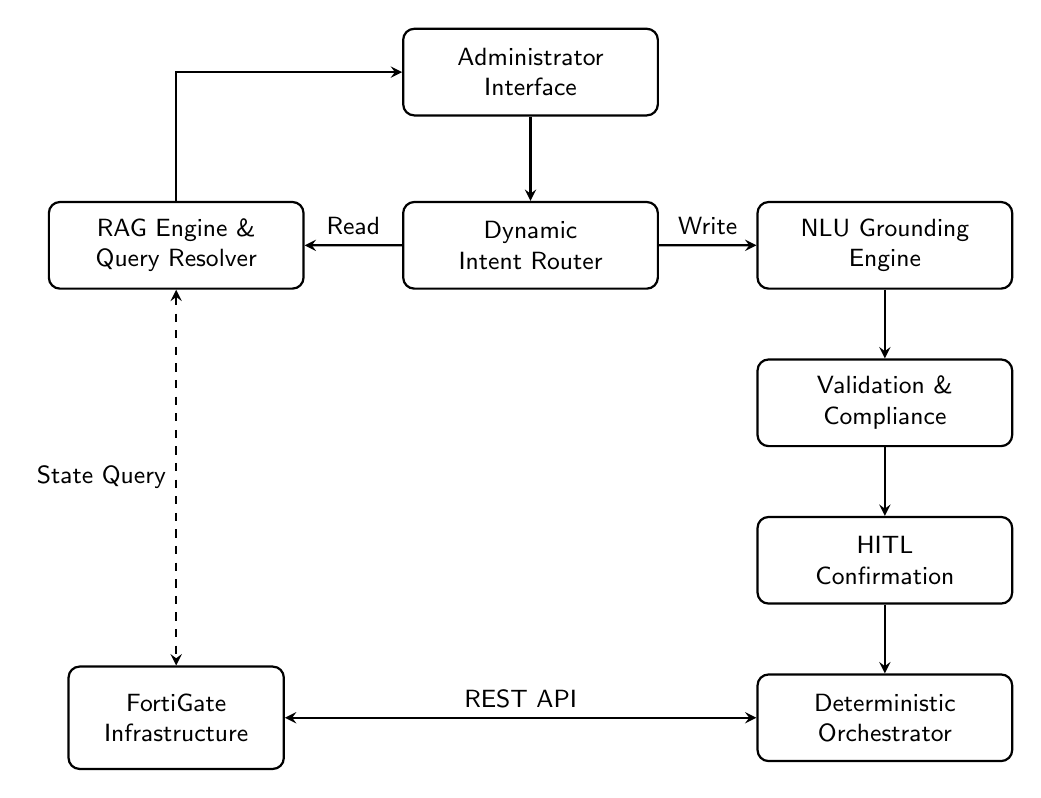
\begin{tikzpicture}[
        node distance=2.2cm,
        every node/.style={font=\sffamily\small},
        component/.style={rectangle, draw=black, thick, fill=white, text width=3.0cm, align=center, minimum height=1.1cm, rounded corners},
        database/.style={rectangle, draw=black, thick, fill=white, text width=2.5cm, align=center, minimum height=1.3cm, rounded corners},
        arrow/.style={->, thick, draw=black, >=stealth}
        ]
        
        % Symmetrical Layout Nodes
        \node[component, fill=white] (user) at (0, 0) {Administrator\\Interface};
        \node[component, below of=user, node distance=2.2cm] (router) {Dynamic\\Intent Router};
        
        % Left Side: Read-Only Path
        \node[component] (rag) at (-4.5, -2.2) {RAG Engine \&\\Query Resolver};
        \node[database] (fortigate) at (-4.5, -8.2) {FortiGate\\Infrastructure};
        
        % Right Side: Write Mutation Path
        \node[component] (grounding) at (4.5, -2.2) {NLU Grounding\\Engine};
        \node[component] (validator) at (4.5, -4.2) {Validation \&\\Compliance};
        \node[component] (hitl) at (4.5, -6.2) {HITL\\Confirmation};
        \node[component] (executor) at (4.5, -8.2) {Deterministic\\Orchestrator};
        
        % Orderly Connections (No Crossings)
        \draw[arrow] (user) -- (router);
        \draw[arrow] (router) -- node[above] {Read} (rag);
        \draw[arrow] (router) -- node[above] {Write} (grounding);
        \draw[arrow] (rag) |- (user);
        \draw[arrow] (grounding) -- (validator);
        \draw[arrow] (validator) -- (hitl);
        \draw[arrow] (hitl) -- (executor);
        \draw[arrow, <->] (executor) -- node[above] {REST API} (fortigate);
        \draw[arrow, <->, dashed] (rag) -- node[left] {State Query} (fortigate);
        
    \end{tikzpicture}
    \caption{Global Platform Architecture and Component Interaction}
    \label{fig:global_arch}
\end{figure}

One important part of this design is to establish hard \textbf{trust boundaries}. All outputs of probabilistic language models are treated as \textbf{unvalidated data} by the system until they pass the \textbf{deterministic validation threshold}. This is in line with the interactive machine learning paradigm explored by Gómez-Carmona et al. \cite{gomez2024hitl}, which aims to keep the human in the loop to review and validate complex decisions, so that automated systems can be kept safe, interpretable, and under tight human supervision.

\begin{figure}[H]
    \centering
    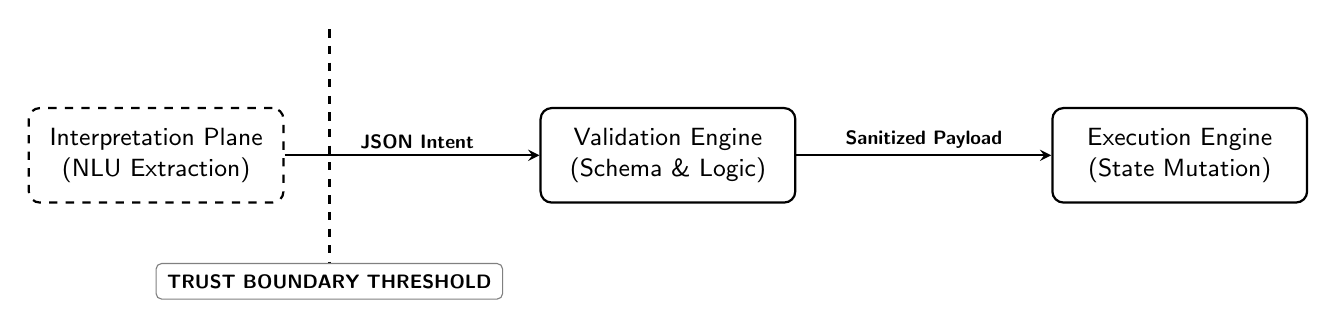
\begin{tikzpicture}[
        node distance=2.5cm,
        every node/.style={font=\sffamily\small},
        untrusted/.style={rectangle, draw=black, thick, dashed, fill=white, text width=3.0cm, align=center, minimum height=1.2cm, rounded corners},
        trusted/.style={rectangle, draw=black, thick, fill=white, text width=3.0cm, align=center, minimum height=1.2cm, rounded corners},
        arrow/.style={->, thick, draw=black, >=stealth},
        badge/.style={fill=white, font=\sffamily\scriptsize\bfseries, inner sep=2pt}
        ]
        
        % Symmetrical and Widened Node Placements (6.5cm center-to-center distance)
        \node[untrusted] (llm) at (0, 0) {Interpretation Plane\\(NLU Extraction)};
        \node[trusted] (val) at (6.5, 0) {Validation Engine\\(Schema \& Logic)};
        \node[trusted] (exec) at (13.0, 0) {Execution Engine\\(State Mutation)};
        
        % Vertical Boundary Line perfectly positioned at x = 2.2
        \draw[black, very thick, dashed] (2.2, 1.6) -- (2.2, -1.6);
        
        % Clean Monochrome Boundary Label at the Bottom, aligned at x = 2.2
        \node[draw=black!50, fill=white, rounded corners=2pt, font=\sffamily\scriptsize\bfseries, inner sep=4pt] at (2.2, -1.6) {TRUST BOUNDARY THRESHOLD};
        
        % Connections with perfect middle-right positioning (Zero overlapping)
        \draw[arrow] (llm) -- node[above, pos=0.52, badge] {JSON Intent} (val);
        \draw[arrow] (val) -- node[above, pos=0.5, badge] {Sanitized Payload} (exec);
        
    \end{tikzpicture}
    \caption{Trust Boundary Architecture separating Interpretation and Control Planes}
    \label{fig:trust_boundary}
\end{figure}

\section{Conceptual Routing \& Intent Flow}
The platform is designed with a dynamic intent routing architecture that enables interaction with infrastructure and guarantees the safety of operations. The router does not give equal treatment to all conversational inputs, but classifies the intent to enforce structural \textbf{Read/Write operational isolation}.

\begin{table}[H]
    \centering
    \caption{Intent Classification and Routing Architecture}
    \label{tab:routing_class}
    \renewcommand{\arraystretch}{1.5}
    \small
    \begin{tabular}{|l|p{5cm}|p{6.5cm}|}
        \hline
        \textbf{Operation Class} & \textbf{Routing Destination} & \textbf{Architectural Objective} \\
        \hline
        \textbf{State Query} & Live API Read Engine & Retrieve current interface status, active policies, or system health directly from the infrastructure. \\
        \hline
        \textbf{Knowledge Query} & RAG Reference Engine & Query indexed Fortinet documentation to assist the administrator. \\
        \hline
        \textbf{Mutation Request} & NLU Grounding Pipeline & Extract structured intent for creating, modifying, or deleting operational configurations. \\
        \hline
        \textbf{Ambiguous Intent} & Clarification Loop & Reject vague requests and logically prompt the user for mandatory operational parameters. \\
        \hline
    \end{tabular}
\end{table}

\section{High-Level Grounding Concepts}
A primary engineering issue encountered in intent-based orchestration systems is converting vague human references into strict infrastructure identifiers. This semantic conversion process is accomplished by the \textbf{Grounding Engine}. For instance, if an administrator requests to "block traffic from the web servers," then the NLU will extract the entity concept. Following this extraction, the deterministic \textbf{reconciliation engine} queries the live FortiGate state to obtain the exact address object names or IP subnets needed by the underlying API corresponding to "web servers."

If an entity cannot be definitively resolved against the live infrastructure state, or if required operational parameters are missing, the system initiates a \textbf{Conversational Clarification Loop}. This workflow ensures the platform behaves as a collaborative administrative assistant, persistently requesting specific context until the intent is deterministically sound.

\section{Operational Processing Pipeline}
To ensure deterministic execution, every mutation request traverses a rigorous operational lifecycle. This pipeline acts as a sequential state machine, guiding an administrative request from its initial natural language ingestion, through entity grounding and human-in-the-loop review, down to the final REST API orchestration and verification. The deeply technical execution mechanics of this lifecycle, including the multi-phase transition matrix, are explored extensively in Chapter 3.

\section{Validation \& Compliance Strategy}
Before any configuration payload reaches the execution layer, it is subjected to a multi-tiered validation strategy. This strategy enforces structural integrity (syntactic checking), dynamic reconciliation (semantic grounding), and strict organizational security postures (proactive compliance). By validating intents conceptually before they are executed physically, the platform prevents misconfigurations. The mathematical logic driving these compliance gates is detailed in the architectural design sections of Chapter 3.

\section{Infrastructure Lifecycle Management}
While conversational interpretation forms the probabilistic layer of the platform, robust infrastructure-as-code principles mandate fail-safe execution mechanics. Network configurations are intrinsically stateful; partial API updates can inadvertently sever remote administrative access. Consequently, the platform embeds snapshot and state-restoration (rollback) protocols natively into the orchestration engine. This guarantees transaction-like safety for all administrative modifications, the programmatic implementation of which is analyzed in Chapter 3.

\section{Methodology and Task Distribution}
The project was executed utilizing an \textbf{Agile engineering methodology}, incorporating iterative sprints to progressively build, integrate, and harden the architecture. This approach facilitated the continuous refinement of the conversational interface while rigorously testing the deterministic API orchestration against simulated enterprise topologies.

\begin{table}[H]
    \centering
    \caption{Agile Development Phases and Project Milestones}
    \label{tab:project_phases}
    \renewcommand{\arraystretch}{1.5}
    \small
    \begin{tabular}{|p{3.5cm}|p{9cm}|}
        \hline
        \textbf{Engineering Phase} & \textbf{Core Deliverables and Focus Areas} \\
        \hline
        \textbf{Architecture Design} & State of the art analysis, system modeling, defining trust boundaries, and read/write separation models. \\
        \hline
        \textbf{API Orchestration} & Development of the deterministic Python backend, state synchronization, snapshot, and restoration modules. \\
        \hline
        \textbf{Intelligence Layer} & Implementation of the NLU grounding pipeline, entity reconciliation, and the intent routing architecture. \\
        \hline
        \textbf{Workflow Refinement} & Integration of the clarification loop, HITL interfaces, and proactive compliance enforcement. \\
        \hline
        \textbf{Validation} & Comprehensive system testing, latency optimization, and verification against complex edge-case network scenarios. \\
        \hline
    \end{tabular}
\end{table}

\section{Project Planning}
The implementation and orchestration of this graduation project were arranged in a sequential manner to address the critical dependencies between the deterministic execution layers and probabilistic conversational interfaces. A first engineering phase focused on developing and hardening the deterministic Python orchestration engine, with all API bindings, state recovery snapshots and verification pipelines thoroughly tested. NLU grounding layer and RAG capabilities were then combined and deployed Human-in-the-Loop (HITL) workflow and conversational clarification loops.

The project was divided into five discrete phases in order with a total of 12 weeks (3 months) duration for professional engineering and strict schedule follow-up. Figure~\ref{fig:project_roadmap} shows the roadmap of the visual execution. The vertical waterfall of engineering sprints and the dashed trigger points for core project milestones.

\begin{figure}[H]
    \centering
    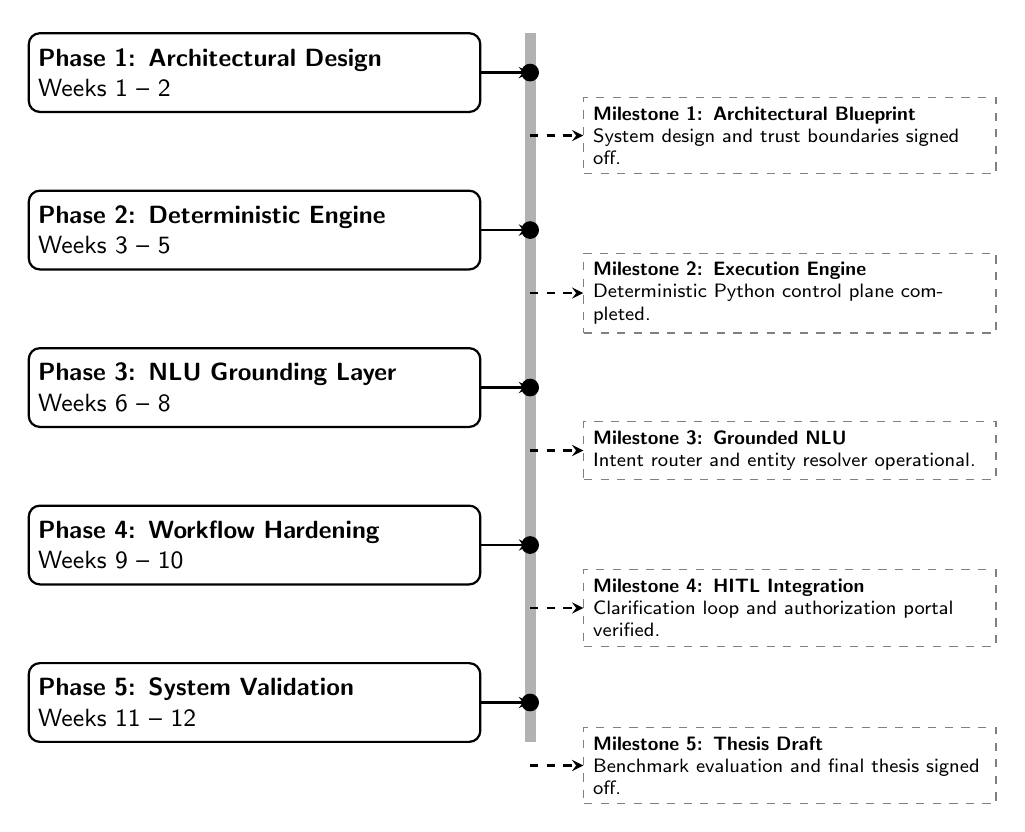
\begin{tikzpicture}[
        node distance=1.5cm,
        every node/.style={font=\sffamily\small},
        phase/.style={rectangle, draw=black, thick, fill=white, text width=5.5cm, align=left, minimum height=1.0cm, rounded corners},
        milestone/.style={rectangle, draw=black!50, dashed, fill=white, text width=5.0cm, align=left, font=\sffamily\scriptsize},
        arrow/.style={->, thick, draw=black, >=stealth}
        ]
        
        % Vertical timeline track
        \draw[black!30, line width=4pt] (0, 0.5) -- (0, -8.5);
        
        % Phase Nodes (Left of track)
        \node[phase] (p1) at (-3.5, 0) {\textbf{Phase 1: Architectural Design}\\Weeks 1 -- 2};
        \node[phase] (p2) at (-3.5, -2.0) {\textbf{Phase 2: Deterministic Engine}\\Weeks 3 -- 5};
        \node[phase] (p3) at (-3.5, -4.0) {\textbf{Phase 3: NLU Grounding Layer}\\Weeks 6 -- 8};
        \node[phase] (p4) at (-3.5, -6.0) {\textbf{Phase 4: Workflow Hardening}\\Weeks 9 -- 10};
        \node[phase] (p5) at (-3.5, -8.0) {\textbf{Phase 5: System Validation}\\Weeks 11 -- 12};
        
        % Milestone Nodes (Right of track)
        \node[milestone] (m1) at (3.3, -0.8) {\textbf{Milestone 1: Architectural Blueprint}\\System design and trust boundaries signed off.};
        \node[milestone] (m2) at (3.3, -2.8) {\textbf{Milestone 2: Execution Engine}\\Deterministic Python control plane completed.};
        \node[milestone] (m3) at (3.3, -4.8) {\textbf{Milestone 3: Grounded NLU}\\Intent router and entity resolver operational.};
        \node[milestone] (m4) at (3.3, -6.8) {\textbf{Milestone 4: HITL Integration}\\Clarification loop and authorization portal verified.};
        \node[milestone] (m5) at (3.3, -8.8) {\textbf{Milestone 5: Thesis Draft}\\Benchmark evaluation and final thesis signed off.};
        
        % Horizontal marker circles on track
        \filldraw[black] (0, 0) circle (3pt);
        \filldraw[black] (0, -2.0) circle (3pt);
        \filldraw[black] (0, -4.0) circle (3pt);
        \filldraw[black] (0, -6.0) circle (3pt);
        \filldraw[black] (0, -8.0) circle (3pt);
        
        % Connection lines
        \draw[arrow] (p1.east) -- (0, 0);
        \draw[arrow] (p2.east) -- (0, -2.0);
        \draw[arrow] (p3.east) -- (0, -4.0);
        \draw[arrow] (p4.east) -- (0, -6.0);
        \draw[arrow] (p5.east) -- (0, -8.0);
        
        \draw[arrow, dashed] (0, -0.8) -- (m1.west);
        \draw[arrow, dashed] (0, -2.8) -- (m2.west);
        \draw[arrow, dashed] (0, -4.8) -- (m3.west);
        \draw[arrow, dashed] (0, -6.8) -- (m4.west);
        \draw[arrow, dashed] (0, -8.8) -- (m5.west);
        
    \end{tikzpicture}
    \caption{Project Planning Roadmap: Sprints and Milestone Execution}
    \label{fig:project_roadmap}
\end{figure}

Complementing the visual roadmap, Table~\ref{tab:sprint_planning} outlines the detailed schedule of development sprints, core engineering tasks, and concrete academic deliverables for each phase of the project lifecycle.

\begin{table}[H]
    \centering
    \caption{Project Planning: Sprint Timeline, Tasks, and Key Deliverables}
    \label{tab:sprint_planning}
    \renewcommand{\arraystretch}{1.4}
    \small
    \begin{tabular}{|l|c|p{4.8cm}|p{5.2cm}|}
        \hline
        \textbf{Project Phase} & \textbf{Timeline} & \textbf{Core Tasks \& Sprints} & \textbf{Key Deliverables} \\
        \hline
        \textbf{Phase 1: Architecture} & Weeks 1--2 & Literature review, state-of-the-art analysis, architectural system design. & Sign-off on system architecture and trust boundary definitions. \\
        \hline
        \textbf{Phase 2: Execution} & Weeks 3--5 & Development of deterministic Python REST API wrappers, local state snapshot mechanisms, validation modules. & Fully functional API orchestration control plane with rollback capabilities. \\
        \hline
        \textbf{Phase 3: NLU Layer} & Weeks 6--8 & Intent router training, entity extraction models, RAG vector database indexing for technical documentation. & Trained intent router and operational RAG-assisted knowledge query resolver. \\
        \hline
        \textbf{Phase 4: Workflow} & Weeks 9--10 & Human-in-the-Loop web portal integration, conversation clarification loops, policy verification hooks. & Dual-interface (Streamlit admin panel and HITL approval portal) fully coupled with backend. \\
        \hline
        \textbf{Phase 5: Validation} & Weeks 11--12 & Synthetic load testing, latency benchmarking, configuration error recovery checks, final report writing. & Complete benchmark analysis, performance evaluation metrics, and thesis submission. \\
        \hline
    \end{tabular}
\end{table}

\section{Report Organization}
The remainder of this thesis is structured as follows:
\begin{itemize}
    \item \textbf{Chapter 2: State of the Art and Theoretical Background:} Explores modern infrastructure automation, the evolution of Intent-Based Networking (IBN), and the integration of conversational interfaces in systems engineering.
    \item \textbf{Chapter 3: System Design and Architecture:} Details the conceptual, structural, and detailed design of the system, including the routing engine, entity grounding, validation compliance algorithms, and UML diagrams.
    \item \textbf{Chapter 4: Implementation, Testing, and Validation:} Showcases the implementation environment, the Streamlit user interface, experimental test cases (grounding, compliance blocks, and rollbacks), performance results, and system limitations.
\end{itemize}

\section{Chapter Conclusion}
The introduction to the subject matter and engineering scope of the project is the purpose of this chapter. As we assessed the complexity of today's infrastructure management, we discovered an \textbf{operational gap} (i.e., not to be confused with gaps related to processes) where the degree of flexibility of conversational AI does not meet the degree of dependability required for professional orchestration in this context. Through a well-developed \textbf{hybrid architectural solution}, this platform addresses the gap between the operational flexibility of conversational artificial intelligence (AI) and the absolute dependability of professional orchestration (a case study in the previous section of the introduction section of this document) by creating a secure operational assistant that leverages technology to provide \textbf{controlled routing}, \textbf{accurate object grounding} (which the next chapter covers), \textbf{live state reconciliation}, and \textbf{deterministic validation}.

The \textbf{rigorous lifecycle management processes} incorporated into the platform (i.e., \textbf{compliance}, \textbf{Human-in-the-Loop (HITL) authorization}, and \textbf{validation}) lend themselves to improving the use of natural language to manage enterprise security architectures while protecting the integrity of these systems in a deterministic manner. The following chapters will provide a more in-depth look at the theoretical approaches and implementation technologies that will enable the next generation of orchestration platforms to be operationalized.

\chapter{State of the Art and Theoretical Background}

\section{Introduction}
The design of an intelligent, safe, and conversational orchestration agent for enterprise firewalls requires a rigorous mastery of two intertwined disciplines: modern network administration automation and the controlled integration of artificial intelligence in critical systems. The primary objective of this chapter is to establish a structured theoretical foundation and conduct a comparative analysis of available technologies, culminating in a formally justified selection of the technical stack adopted in this project.

First, we introduce the fundamental theoretical concepts that underpin the project, covering the historical evolution of network administration paradigms, the specific engineering challenges of stateful firewall automation, and the role of key AI constructs — LLMs, RAG, and HITL safeguards. We then contrast the proposed hybrid orchestration model against existing paradigms to motivate the architectural direction. We follow with a detailed presentation of the generic architecture and functioning of a Hybrid AI Orchestration Agent, establishing a clear conceptual model that bridges theory to implementation. Finally, we conduct a structured comparative analysis of available technical solutions, formally justifying the technology stack selected for this project.

%% -----------------------------------------------------------
\section{Fundamental Theoretical Concepts}
%% -----------------------------------------------------------
The realization of a safe, AI-driven network administration agent relies on several interconnected disciplines. This section establishes each individually, building a progressive conceptual foundation.

\subsection{Evolution of Network Administration Paradigms}
Network infrastructure administration has historically evolved through three major paradigm shifts, driven by the growing complexity and scale of enterprise environments, as illustrated in Figure~\ref{fig:admin_evolution}.

\begin{figure}[htbp]
    \centering
    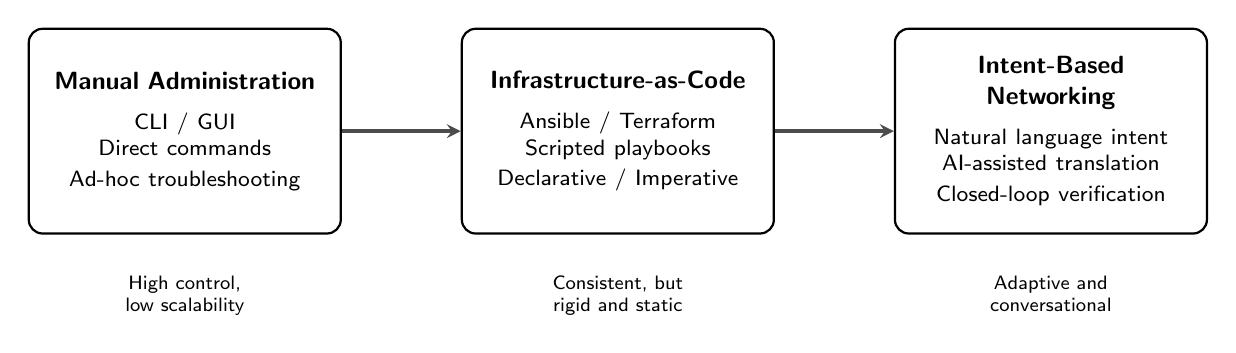
\begin{tikzpicture}[
        every node/.style={font=\sffamily\small},
        era/.style={rectangle, draw=black, thick, fill=white, text width=3.4cm, align=center, minimum height=2.6cm, rounded corners=5pt, inner sep=8pt},
        arrow/.style={->, very thick, draw=black!70, >=stealth},
        sublabel/.style={font=\sffamily\scriptsize, align=center, text width=3.2cm},
    ]
        \node[era] (manual) at (0, 0) {
            \textbf{Manual Administration}\\[5pt]
            \footnotesize CLI / GUI\\
            \footnotesize Direct commands\\
            \footnotesize Ad-hoc troubleshooting
        };
        \node[era] (iac) at (5.5, 0) {
            \textbf{Infrastructure-as-Code}\\[5pt]
            \footnotesize Ansible / Terraform\\
            \footnotesize Scripted playbooks\\
            \footnotesize Declarative / Imperative
        };
        \node[era] (ibn) at (11.0, 0) {
            \textbf{Intent-Based Networking}\\[5pt]
            \footnotesize Natural language intent\\
            \footnotesize AI-assisted translation\\
            \footnotesize Closed-loop verification
        };

        \draw[arrow] (manual.east) -- (iac.west);
        \draw[arrow] (iac.east) -- (ibn.west);

        \node[sublabel, below=0.4cm of manual] {High control,\\low scalability};
        \node[sublabel, below=0.4cm of iac] {Consistent, but\\rigid and static};
        \node[sublabel, below=0.4cm of ibn] {Adaptive and\\conversational};

    \end{tikzpicture}
    \caption{Evolution of Network Administration Paradigms}
    \label{fig:admin_evolution}
\end{figure}

\textbf{Manual Administration} relies on direct interaction via command-line interfaces (CLIs) or graphical interfaces. Although flexible for ad-hoc troubleshooting, manual processes fail to scale and place a severe cognitive burden on administrators, frequently resulting in configuration drift and costly human-induced outages~\cite{benson2009network,oppenheimer2003why}.

\textbf{Infrastructure-as-Code (IaC)} addressed these limitations by introducing a programmatic approach to resource provisioning. The IaC paradigm separates into two primary models: the \emph{imperative} model, where the administrator defines the exact sequence of commands required to reach the desired state (e.g., Ansible playbooks); and the \emph{declarative} model, where the administrator defines the desired final state, leaving the engine to compute the required delta~\cite{hashicorp_terraform} (e.g., Terraform). 

Despite these advancements, both IaC models remain static and cannot dynamically interpret the intent behind a conversational administrative request, nor adapt when live device state diverges from the template.

\textbf{Intent-Based Networking (IBN)} represents the emerging paradigm, where the administrator expresses high-level business or security intent in natural language, and the system autonomously translates, validates, and applies the corresponding configuration. 

According to Leivadeas and Falkner~\cite{leivadeas2022survey}, a mature IBN system operates on a closed-loop feedback model: intent is captured, translated into device configurations, the resulting state is verified against the intended outcome, and deviations are automatically remediated.

\subsection{Specific Challenges of Stateful Firewall Automation}
Firewall automation differs fundamentally from generic cloud resource orchestration. While provisioning a virtual machine is largely order-independent, managing security policies on a stateful firewall appliance introduces strict operational constraints that any automated agent must rigorously address~\cite{alshaer2004discovery}:

\begin{itemize}
    \item \textbf{Policy Ordering and Rule Shadowing:} Firewall Access Control Lists (ACLs) are evaluated in a top-down, first-match order. A broad permissive rule inserted at an incorrect index silently shadows specific restrictive policies, creating undetected security gaps~\cite{yuan2006fireman}.
    \item \textbf{Object Ambiguity and Entity Resolution:} Administrators refer to infrastructure by informal names (e.g., ``the mail server''). An automated agent must rigorously resolve these informal references to live, formal device objects — IP addresses, interface UUIDs, zone names — via active API queries, not static assumptions.
    \item \textbf{Configuration Drift and Out-of-Band Changes:} During security incidents, administrators apply emergency rules directly to the appliance CLI, immediately invalidating any static configuration template. Active state synchronization is therefore not optional — it is a fundamental architectural requirement.
    \item \textbf{Operational Criticality and Blast Radius:} A misconfigured virtual machine affects one host. A misconfigured firewall policy can disconnect entire subnets, sever corporate VPN gateways, or expose critical database segments to the public internet. This elevated blast radius demands rigid pre-execution verification gates before any change is applied.
\end{itemize}

This disconnect — between the abstract, business-driven language of the administrator and the rigid, syntax-heavy configuration commands required by the appliance — constitutes what is commonly referred to as the \textbf{Semantic Gap}. Bridging this gap without sacrificing execution predictability is the primary engineering challenge of modern network automation.

\subsection{Conversational AI: LLMs, RAG, and Safety Constraints}
The emergence of Large Language Models (LLMs) introduces the ability to declare administrative intent in natural language~\cite{boutaba2018comprehensive}. Rather than memorizing proprietary syntax, an administrator can simply describe what they need, and the model translates this into machine-readable instructions.

However, deploying a generic LLM as a direct execution agent over critical infrastructure introduces unacceptable risks. LLMs are inherently \emph{stochastic}: the same prompt may yield different outputs across invocations, and models are known to \emph{hallucinate} — generating plausible-sounding but factually incorrect values such as non-existent IP addresses, deprecated API fields, or invalid interface names~\cite{wang2024netconfeval}. Furthermore, a static language model has no awareness of the live state of the target device.

Two core technical safeguards are therefore mandatory to bridge the gap between the conversational power of LLMs and the rigid safety requirements of network security:

\begin{itemize}
    \item \textbf{Retrieval-Augmented Generation (RAG):} RAG grounds the language model's outputs by coupling it with a curated vector database \cite{lewis2020rag}. Before generating a response, the model retrieves the most semantically relevant technical documentation fragments and uses them as context. In network operations, this ensures that generated API payloads conform to documented schemas and that referenced objects exist on the live device~\cite{shajarian2024rag}.

    \item \textbf{Human-in-the-Loop (HITL) Validation:} Even a grounded LLM cannot guarantee the absence of policy-level errors in a live network context. The HITL paradigm~\cite{gomez2024hitl} positions the human administrator as the mandatory gatekeeper of all state mutations. A deterministic software layer intercepts the AI-generated payload, validates its structural and semantic correctness, presents a verifiable configuration diff to the operator, and awaits explicit approval before any command reaches the physical appliance.
\end{itemize}

Figure~\ref{fig:rag_pipeline} illustrates how RAG enrichment operates conceptually within the AI pipeline, grounding the model's generation with live context before a payload is produced.

\begin{figure}[htbp]
    \centering
    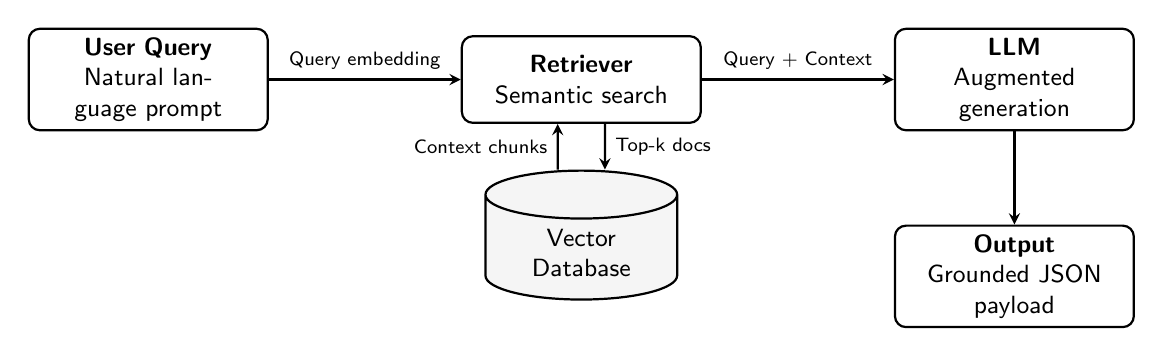
\begin{tikzpicture}[
        every node/.style={font=\sffamily\small},
        box/.style={rectangle, draw=black, thick, fill=white, text width=2.8cm, align=center, minimum height=1.1cm, rounded corners=4pt},
        dbbox/.style={cylinder, draw=black, thick, fill=gray!8, text width=2.2cm, align=center, minimum height=1.0cm, shape border rotate=90, aspect=0.25},
        arrow/.style={->, thick, draw=black, >=stealth},
        label/.style={font=\sffamily\scriptsize},
    ]

        \node[box] (query) at (0, 0) {\textbf{User Query}\\Natural language prompt};
        \node[dbbox] (vdb) at (5.5, -2.2) {Vector\\Database};
        \node[box] (context) at (5.5, 0) {\textbf{Retriever}\\Semantic search};
        \node[box] (llm) at (11.0, 0) {\textbf{LLM}\\Augmented\\generation};
        \node[box] (output) at (11.0, -2.5) {\textbf{Output}\\Grounded JSON\\payload};

        \draw[arrow] (query) -- node[above, label]{Query embedding} (context);
        \draw[arrow, transform canvas={xshift=0.3cm}] (context.south) -- node[right, label]{Top-k docs} (vdb.north);
        \draw[arrow, transform canvas={xshift=-0.3cm}] (vdb.north) -- node[left, label]{Context chunks} (context.south);
        \draw[arrow] (context) -- node[above, label]{Query + Context} (llm);
        \draw[arrow] (llm) -- (output);

    \end{tikzpicture}
    \caption{RAG Pipeline for LLM Grounding}
    \label{fig:rag_pipeline}
\end{figure}

%% -----------------------------------------------------------
\section{Comparative Analysis of Orchestration Models}
%% -----------------------------------------------------------
Having established the theoretical building blocks, it is necessary to contrast the proposed hybrid approach against existing orchestration paradigms before detailing its architecture. This comparison motivates the architectural direction of this project and establishes its unique contribution. Table~\ref{tab:orchestration_models} presents a structured comparison across four critical operational dimensions.

\begin{table}[htbp]
    \small
    \centering
    \renewcommand{\arraystretch}{1.4}
    \begin{tabular}{|p{2.8cm}|p{3.3cm}|p{3.8cm}|p{4.5cm}|}
        \hline
        \textbf{Feature} & \textbf{Static IaC (e.g., Terraform)} & \textbf{Pure LLM Agent} & \textbf{Hybrid Agent (Proposed)} \\
        \hline
        \textbf{Interface} & Code / CLI only & Conversational natural language & Conversational NL with live grounded context \\
        \hline
        \textbf{Safety Model} & Deterministic schema validation & Probabilistic, hallucination-prone~\cite{wang2024netconfeval} & Deterministic validation gate with mandatory HITL~\cite{gomez2024hitl} \\
        \hline
        \textbf{State Sync} & Static file, prone to drift & None --- blind execution & Active live API synchronization with pre-execution snapshots \\
        \hline
        \textbf{Recovery} & Manual destroy and re-apply & None (no rollback) & Automated transaction rollback on detected state drift (custom architecture) \\
        \hline
        \textbf{Adaptability} & None (rigid playbooks) & High (but unsafe) & High and safe (intent-routing with safety gates) \\
        \hline
    \end{tabular}
    \caption{Comparison of Network Orchestration Models}
    \label{tab:orchestration_models}
\end{table}

The hybrid model uniquely combines the conversational flexibility of LLM interfaces with the execution-time guarantees of a deterministic control plane. This synthesis motivates the architectural pattern formally defined in the following section.

%% -----------------------------------------------------------
\section{Theoretical Necessity of a Hybrid Architecture}
%% -----------------------------------------------------------
The preceding theoretical analysis converges on a single architectural necessity: the \textbf{Hybrid AI Network Orchestration Model}. This section formalizes the concept of a hybrid model, detailing why the isolation of generative inference from rule-based execution is critical for network safety.

\subsection{The Requirement for Execution Isolation}
The integration of generative models into critical infrastructure mandates the coexistence of two operationally distinct domains:

\begin{itemize}
    \item \textbf{Probabilistic Reasoning:} The capacity to parse unstructured natural language, retrieve organizational context, and formulate intended configurations. This domain relies on non-deterministic language models.
    \item \textbf{Deterministic Execution:} The capacity to validate syntactic correctness, enforce security policies, and apply state mutations to physical hardware. This domain must rely on rigid, verifiable logic.
\end{itemize}

The core theoretical necessity is that these two domains must never merge. They must be separated by a strict \textbf{Isolation Perimeter}: an architectural boundary that prevents any AI-generated artifact from reaching the network device without first undergoing programmatic verification and explicit human approval. This requirement dictates the transition from standalone AI chat interfaces to a hybrid, defensively engineered orchestration model.

\subsection{Redefining the Administrator's Role}
The adoption of a hybrid orchestration agent fundamentally redefines the operational responsibilities of the human administrator. Rather than eliminating the human from the process, the system strategically re-assigns tasks to maximize both operational velocity and safety guarantees. Table~\ref{tab:roles_actors} formally defines these reassigned responsibilities.

\begin{table}[htbp]
    \small
    \centering
    \renewcommand{\arraystretch}{1.5}
    \begin{tabular}{|p{4.0cm}|p{5.5cm}|p{5.0cm}|}
        \hline
        \textbf{Responsibility} & \textbf{Traditional Manual Admin} & \textbf{With AI Orchestration Agent} \\
        \hline
        \textbf{Intent Formulation} & Translates intent into CLI syntax manually & Expresses intent in natural language \\
        \hline
        \textbf{Configuration Drafting} & Writes commands directly & Delegated entirely to the AI Agent \\
        \hline
        \textbf{Safety Verification} & Performed manually (error-prone) & Automated by the Validation Engine \\
        \hline
        \textbf{Change Approval} & Implicit (execution = approval) & Explicit HITL confirmation required \\
        \hline
        \textbf{State Recovery} & Manual diagnosis and rollback & Automatic snapshot-based rollback \\
        \hline
        \textbf{Audit Trail} & Depends on manual logging discipline & Cryptographically appended audit log \\
        \hline
    \end{tabular}
    \caption{Operational Responsibilities Distribution}
    \label{tab:roles_actors}
\end{table}

The administrator's role is elevated from low-level syntax specialist to high-level intent decision-maker and safety authority. The AI agent absorbs the repetitive, syntactically intensive work, while the human retains ultimate authority over every state mutation applied to the live network.

%% -----------------------------------------------------------
\section{Comparative Analysis of Technical Solutions}
%% -----------------------------------------------------------
The choice of tools and technologies constitutes a critical engineering decision for each functional layer of the agent. This section analyzes the principal solutions available on the market and formally justifies the selection made for this project.

\subsection{Large Language Models (LLMs)}
The NLU engine requires a model capable of strictly following structured system instructions, producing syntactically correct JSON payloads, and operating with minimal latency for real-time conversational interactions. Three representative models were evaluated.

\begin{table}[htbp]
    \small
    \centering
    \renewcommand{\arraystretch}{1.4}
    \begin{tabular}{|p{3.0cm}|p{3.5cm}|p{3.5cm}|p{3.8cm}|}
        \hline
        \textbf{Criterion} & \textbf{OpenAI GPT-4} & \textbf{Meta Llama 3 (8B)} & \textbf{Mistral (mistral-small)} \\
        \hline
        \textbf{Deployment Mode} & Cloud API only & Local self-hosted & Cloud API or local \\
        \hline
        \textbf{JSON Schema Adherence} & Excellent (native function calling) & Requires extensive prompt engineering & Native strict JSON output mode \\
        \hline
        \textbf{API Response Latency} & Moderate (large model overhead) & Fast (GPU-dependent) & Very fast via lightweight API \\
        \hline
        \textbf{Cost Model} & High per-token pricing & Free (hardware cost only) & Highly cost-effective \\
        \hline
    \end{tabular}
    \caption{Comparison of LLMs for Intent Parsing}
    \label{tab:llm_comparison}
\end{table}

\textbf{Mistral AI (mistral-small-latest)} was selected. Its native JSON output mode enforces structured schema adherence at the model level, eliminating the risk of malformed payloads reaching the validation gate. Its very low inference latency makes it well-suited for real-time conversational interactions, and its cost-effective API pricing is appropriate for an academic engineering prototype requiring numerous validation test cycles.

\subsection{Vector Databases for the RAG Pipeline}
The RAG module requires a vector database capable of storing embedded documentation fragments and device object references, supporting fast semantic similarity search with no dependency on external cloud infrastructure.

\begin{table}[htbp]
    \small
    \centering
    \renewcommand{\arraystretch}{1.4}
    \begin{tabular}{|p{3.0cm}|p{3.5cm}|p{3.5cm}|p{3.8cm}|}
        \hline
        \textbf{Criterion} & \textbf{Pinecone} & \textbf{Qdrant} & \textbf{ChromaDB} \\
        \hline
        \textbf{Architecture} & Managed Cloud SaaS & Rust-based client/server & Python-native, embeddable \\
        \hline
        \textbf{Deployment} & External cloud, API keys required & Self-hosted via Docker & Zero-config embedded or containerized \\
        \hline
        \textbf{Data Sovereignty} & Data leaves the local network & Can be fully self-hosted & Fully local and persistent \\
        \hline
        \textbf{Python Integration} & REST API client library & REST API client library & Direct Python package import \\
        \hline
    \end{tabular}
    \caption{Comparison of Vector Databases}
    \label{tab:vector_db}
\end{table}

\textbf{ChromaDB} was selected for its Python-native architecture. It can operate in an embedded mode alongside the orchestrator or as a lightweight containerized service, requiring no external cloud infrastructure. All indexed FortiOS API documentation and device object references remain within the local environment, guaranteeing full data sovereignty for sensitive network inventory data.

\subsection{Backend Execution Framework}
The deterministic execution plane must dynamically construct, validate, and dispatch REST API calls to the FortiGate appliance based on the AI-generated payload received at runtime.

\begin{table}[htbp]
    \small
    \centering
    \renewcommand{\arraystretch}{1.4}
    \begin{tabular}{|p{3.0cm}|p{3.5cm}|p{3.5cm}|p{3.8cm}|}
        \hline
        \textbf{Criterion} & \textbf{Ansible (RedHat)} & \textbf{Nornir} & \textbf{Custom Python (httpx)} \\
        \hline
        \textbf{Execution Model} & Static YAML playbooks & Pluggable task execution & Synchronous/async HTTP client \\
        \hline
        \textbf{Dynamic JSON Handling} & Poor (static variable templating) & Moderate (requires plugin) & Excellent (full Python runtime) \\
        \hline
        \textbf{REST API Throughput} & Low (SSH-based overhead) & High (concurrent workers) & High (connection pooling, async I/O) \\
        \hline
        \textbf{Programmatic Flexibility} & Limited (no runtime branching logic) & Good & Full (native Python control flow) \\
        \hline
    \end{tabular}
    \caption{Comparison of Backend Frameworks}
    \label{tab:backend_frameworks}
\end{table}

A \textbf{custom Python orchestration engine using the httpx library} was selected as the REST client layer. While dedicated network automation frameworks like Ansible or Nornir excel at bulk configuration templating, they introduce unnecessary overhead when bridging dynamic AI JSON outputs directly to REST APIs. Python provides complete programmatic flexibility. The \texttt{httpx} library enables both synchronous and asynchronous HTTPS calls to the FortiOS REST API, supporting connection pooling and configurable timeouts — critical for reliably detecting management connectivity loss during post-execution verification.

\subsection{User Interface for the Security Operations Dashboard}
The Human-in-the-Loop confirmation workflow requires a dashboard interface that presents configuration diffs clearly, collects explicit operator approval, and provides real-time visibility into agent state.

\begin{table}[htbp]
    \small
    \centering
    \renewcommand{\arraystretch}{1.4}
    \begin{tabular}{|p{3.0cm}|p{3.5cm}|p{3.5cm}|p{3.8cm}|}
        \hline
        \textbf{Criterion} & \textbf{React / Node.js} & \textbf{Gradio} & \textbf{Streamlit} \\
        \hline
        \textbf{Implementation Language} & JavaScript / TypeScript & Python & Python \\
        \hline
        \textbf{Development Velocity} & Low (requires dedicated frontend) & Very high (limited customization) & High (flexible layout controls) \\
        \hline
        \textbf{Backend Integration} & Requires REST API bridge layer & Direct Python integration & Direct Python integration \\
        \hline
        \textbf{UI Customization} & Unlimited & Minimal & High (custom CSS, dynamic layouts) \\
        \hline
    \end{tabular}
    \caption{Comparison of UI Frameworks}
    \label{tab:ui_frameworks}
\end{table}

\textbf{Streamlit} was selected as the dashboard framework. It allows the rapid construction of interactive, Python-native web applications with direct access to the backend validation and session management logic. Its support for custom CSS injection, dynamic column layouts, and dark-mode theming produces a professional, SOC-appropriate dashboard aesthetic without requiring a separate JavaScript codebase or a REST API bridge layer.

\subsection{Target Network Appliance: The Firewall Ecosystem}
The target appliance must expose a comprehensive, programmatically accessible API permitting granular manipulation of security policies, address objects, NAT rules, and routing entries — without requiring a separate, mandatory management server.

\begin{table}[htbp]
    \small
    \centering
    \renewcommand{\arraystretch}{1.4}
    \begin{tabular}{|p{3.0cm}|p{3.5cm}|p{3.5cm}|p{3.8cm}|}
        \hline
        \textbf{Criterion} & \textbf{Cisco ASA} & \textbf{Palo Alto Networks} & \textbf{Fortinet FortiGate} \\
        \hline
        \textbf{API Accessibility} & Legacy REST API (often requires ASDM) & Excellent XML/REST API & Modern, granular REST API \\
        \hline
        \textbf{Management Model} & Standalone or FMC & Often relies on Panorama & Fully standalone capable \\
        \hline
        \textbf{Local Testing VM} & Available (ASAv) & Heavy resource requirements & Lightweight FortiOS VM available \\
        \hline
    \end{tabular}
    \caption{Comparison of Firewall Appliances}
    \label{tab:firewall_appliances}
\end{table}

\textbf{Fortinet FortiGate} running \textbf{FortiOS} was selected as the target appliance. While competitors like Palo Alto offer excellent APIs, they frequently rely on centralized management platforms (like Panorama) for complex orchestration. The FortiOS REST API provides a complete, well-documented interface for managing all network objects via token-authenticated HTTPS requests directly against the standalone appliance. This makes it ideally suited for an orchestration agent that must synchronize live state and apply precise mutations in real time. Furthermore, Fortinet's provision of a free FortiGate Virtual Machine edition enabled the establishment of a fully isolated local hypervisor environment for development and validation.

%% -----------------------------------------------------------
\section{Chapter Conclusion}
%% -----------------------------------------------------------
This chapter has progressively established the complete theoretical and technological foundation required for the realization of the hybrid AI orchestration agent. Starting from the cognitive burden of manual firewall administration and the rigid limitations of static IaC frameworks, the chapter built the case for a new operational paradigm grounded in Intent-Based Networking principles and AI-assisted natural language understanding.

The generic anatomy and functioning of a Hybrid AI Orchestration Agent were formally defined and illustrated: a system structured around four functional components operating across a strict Trust Boundary, through which every administrative request must travel from natural language input to deterministic, human-approved execution. The redistribution of operational responsibilities between administrator and agent was also formalized, highlighting the elevation of the human role from syntax specialist to intent authority and safety gatekeeper.

Finally, the comparative analysis of available technologies culminated in the formal justification of the selected stack: Mistral AI for intent parsing, ChromaDB for grounded RAG retrieval, Python with httpx for deterministic execution, Streamlit for the HITL dashboard, and FortiGate for the target appliance ecosystem.

With this foundation established, the following chapter will present the detailed system design and architectural blueprint of the implemented agent, translating these theoretical constructs into concrete software components, UML models, and validation mechanisms.

\chapter{System Design and Architecture}
\markboth{Chapter 3. System Design and Architecture}{Chapter 3. System Design and Architecture}

\section{Introduction}
To bridge the gap between conversational agility and deterministic network infrastructure management, a robust architectural foundation is required. This chapter details the conceptual, structural, and detailed design of our hybrid network orchestration prototype. We translate the theoretical principles of Intent-Based Networking (IBN) established in RFC 9315~\cite{rfc9315} into a concrete software design, isolating the probabilistic natural language processing plane from the deterministic control plane. By grounding our validation rules in classical firewall policy anomaly analysis models such as those proposed by Al-Shaer and Hamed~\cite{alshaer2004discovery} and Yuan et al.~\cite{yuan2006fireman}, we ensure that the hybrid system remains mathematically sound, secure, and fail-safe.

We begin by specifying the functional and non-functional requirements that govern system safety, functionality, and operational performance. We then present the multi-layered block architecture, illustrating the hard trust boundary separating untrusted AI models from verified execution modules. Next, we detail the NLP and RAG Ingestion Pipeline, showcasing the dynamic classifier and semantic vector database enrichment. Finally, we analyze the translation and execution engine, the security compliance safety gates, the transactional state snapshot-rollback lifecycle, and the structural UML models mapping actor interactions and object-oriented class relationships.

\subsection{Transition from Theoretical Frameworks to Architecture}
The theoretical paradigms analyzed in Chapter 2---ranging from declarative Intent-Based Networking (IBN) models to Human-in-the-Loop (HITL) control mechanisms---establish the conceptual requirements for our prototype. However, operationalizing these concepts on physical enterprise hardware requires a concrete software design. This section bridges the theoretical demand for validation gates and trust boundaries with the multi-tiered software architecture described below, detailing our routing modules, grounding engines, session state transition matrices, and UML class designs.

\section{System Requirements and Specifications}
Before translating design principles into software components, we define the strict specifications that govern the system.

\subsection{Functional Requirements}
The functional requirements represent the core capabilities that the orchestrator must perform to assist the network administrator. They are structured into four main operational pillars:
\begin{enumerate}
    \item \textbf{Conversational Interpretation (Read/Write Parsing):} The system must ingest unstructured administrative prompts in English or French, classifying them dynamically into read queries (status, logs, active states) or configuration write intents (policy mutations, object management, system tasks).
    \item \textbf{Contextual Entity Grounding:} The system must dynamically reconcile ambiguous user references (e.g., ``allow public traffic to the mail server'') with active, physical device elements retrieved via live REST API queries (mapping ``mail server'' to its corresponding IP address object and UUID).
    \item \textbf{Deterministic Safety Validation:} The system must perform forward-looking compliance checks, verifying that no policy violates predefined corporate standards (e.g., blocking HTTP/Telnet management or preventing public exposure of insecure ports).
    \item \textbf{Transactional Lifecycle Management:} Before mutating device states, the system must take a complete, localized configuration snapshot. Post-execution, it must verify the active configuration on the physical firewall. If verification fails or communication is severed, the system must automatically execute an inverse rollback to restore the firewall to its pre-state.
\end{enumerate}

\subsection{Non-Functional Requirements}
Non-functional requirements specify the architectural constraints, quality standards, and safety bounds of the implementation:
\begin{itemize}
    \item \textbf{Predictability and Safety:} No configuration modification may be executed directly by a probabilistic model. The AI-assisted interface is strictly restricted to intent parsing, leaving all execution, validation, and API interactions to deterministic Python logic.
    \item \textbf{Operator Oversight (HITL):} All state-mutating transactions require explicit administrative approval. The system must present a side-by-side unified delta diff of the planned changes before requesting confirmation.
    \item \textbf{Auditability and Log Integrity:} Every session interaction, intermediate intent, validation outcome, and API mutation must be recorded in an audit ledger using a rolling SHA-256 hash sequence to detect unauthorized modifications.
    \item \textbf{Latency and Responsiveness:} The intent classification and parsing pipeline must execute within a low-latency threshold, ensuring that typical query resolutions complete in under three seconds to prevent administrator operational delay.
\end{itemize}

\section{Global System Architecture}
The core design principle of our system is the strict, multi-layered segregation of responsibilities, directly addressing the limitations of unconstrained language models highlighted in NetConfEval~\cite{wang2024netconfeval}. We partition the application into two isolated logical zones: the \textbf{Probabilistic Interpretation Plane} (leveraging NLU models and semantic vector indexes) and the \textbf{Deterministic Control Plane} (implemented strictly in Python code using deterministic schemas).

This structural segregation is illustrated in Figure~\ref{fig:trust_boundary_arch}.

\begin{figure}[H]
    \centering
    \makebox[\textwidth][c]{
    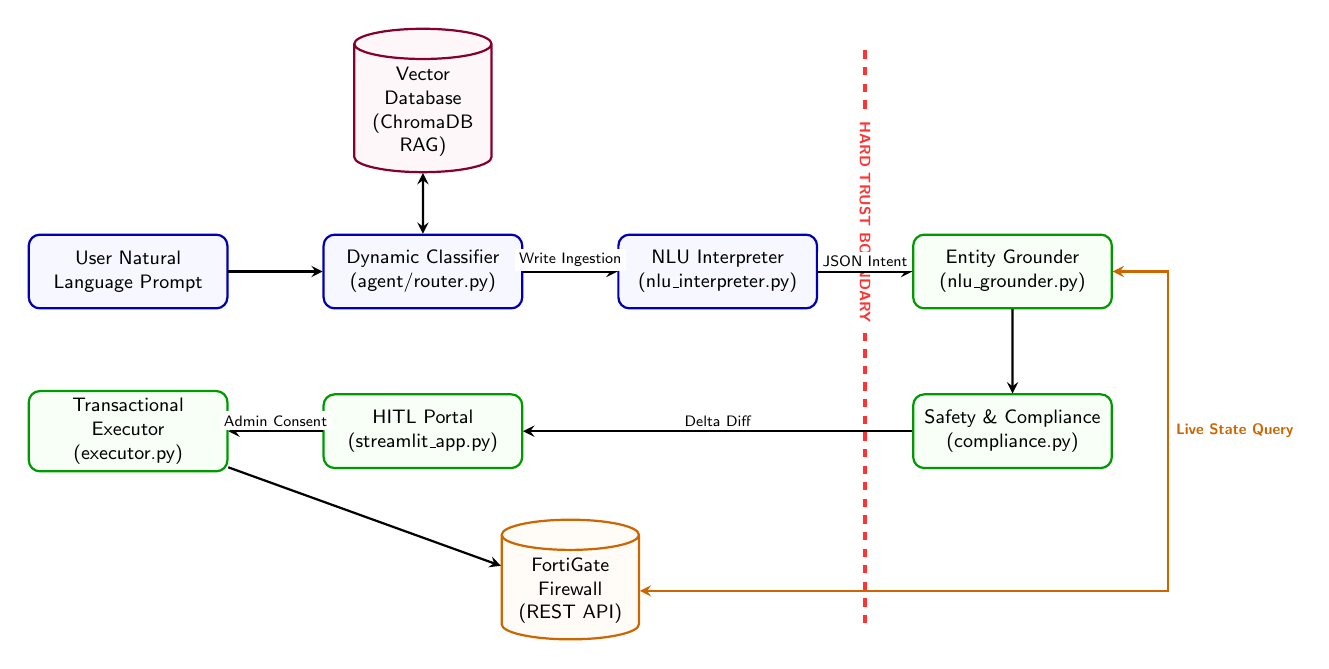
\begin{tikzpicture}[
        scale=0.78, every node/.style={transform shape, font=\sffamily\small},
        blockprob/.style={rectangle, draw=blue!70!black, thick, fill=blue!3, text width=3.0cm, align=center, minimum height=1.2cm, rounded corners},
        blockdet/.style={rectangle, draw=green!60!black, thick, fill=green!3, text width=3.0cm, align=center, minimum height=1.2cm, rounded corners},
        database/.style={cylinder, draw=purple!70!black, thick, fill=purple!3, text width=2.0cm, align=center, minimum height=1.3cm, aspect=0.22, shape border rotate=90},
        firewall/.style={cylinder, draw=orange!80!black, thick, fill=orange!3, text width=2.0cm, align=center, minimum height=1.3cm, aspect=0.22, shape border rotate=90},
        arrow/.style={->, thick, draw=black, >=stealth},
        doublearrow/.style={<->, thick, draw=black, >=stealth},
        boundary/.style={draw=red!70, dashed, ultra thick, fill=red!3, fill opacity=0.05, rounded corners}
        ]
        
        % Probabilistic Zone (Blue Theme)
        \node[blockprob] (user) at (0, 0) {User Natural\\Language Prompt};
        \node[blockprob] (router) at (4.8, 0) {Dynamic Classifier\\(agent/router.py)};
        \node[database] (chroma) at (4.8, 2.6) {Vector Database\\(ChromaDB RAG)};
        \node[blockprob] (nlu) at (9.6, 0) {NLU Interpreter\\(nlu\_interpreter.py)};
        
        % Red Gutter dividing the Trust Boundary (Drawn behind the labels)
        \draw[red!80, dashed, ultra thick] (12.0, 3.6) -- (12.0, -5.8);
        \node[fill=white, inner sep=2pt, rotate=270, text=red!80, font=\sffamily\scriptsize\bfseries] at (12.0, 0.8) {HARD TRUST BOUNDARY};
        
        % Deterministic Zone (Green/Orange Theme)
        \node[blockdet] (ground) at (14.4, 0) {Entity Grounder\\(nlu\_grounder.py)};
        \node[blockdet] (val) at (14.4, -2.6) {Safety \& Compliance\\(compliance.py)};
        \node[blockdet] (hitl) at (4.8, -2.6) {HITL Portal\\(streamlit\_app.py)};
        \node[blockdet] (exec) at (0, -2.6) {Transactional Executor\\(executor.py)};
        
        \node[firewall] (fgt) at (7.2, -5.2) {FortiGate Firewall\\(REST API)};
        
        % Connections
        \draw[arrow] (user) -- (router);
        \draw[doublearrow] (router) -- (chroma);
        \draw[arrow] (router) -- node[above, fill=white, inner sep=2pt, font=\sffamily\scriptsize] {Write Ingestion} (nlu);
        \draw[arrow] (nlu) -- node[above, fill=white, inner sep=2pt, font=\sffamily\scriptsize] {JSON Intent} (ground);
        
        \draw[arrow] (ground) -- (val);
        \draw[arrow] (val) -- node[above, fill=white, inner sep=2pt, font=\sffamily\scriptsize] {Delta Diff} (hitl);
        \draw[arrow] (hitl) -- node[above, fill=white, inner sep=2pt, font=\sffamily\scriptsize] {Admin Consent} (exec);
        \draw[arrow] (exec) -- (fgt);
        
        % Grounder dynamic checking routed around the right side to prevent clashing diagonal lines
        \draw[doublearrow, draw=orange!80!black] (ground.east) -- ++(0.9, 0) |- node[right, pos=0.25, font=\sffamily\scriptsize\bfseries, text=orange!80!black] {Live State Query} (fgt.east);
        
    \end{tikzpicture}
    }
    \caption{Multi-Tiered Block Architecture representing the Hard Trust Boundary}
    \label{fig:trust_boundary_arch}
\end{figure}

The \textbf{Trust Boundary} defines the exact line where probabilistic parsing terminates and deterministic verification begins. Once the NLU Interpreter generates a structured intermediate representation, the AI model is completely suspended, and the Python control plane assumes full execution authority. This prevents LLM hallucinations from ever manifesting as physical device mutations.

\section{The NLP and RAG Ingestion Pipeline}
The system entry point is managed entirely within the Probabilistic Interpretation Plane. The user's unstructured natural language prompt must be parsed and augmented with highly specific technical context before any system intent is generated.

This ingestion flow is structured as a two-stage routing and context enrichment pipeline, as illustrated in Figure~\ref{fig:rag_pipeline}.

\begin{figure}[H]
    \centering
    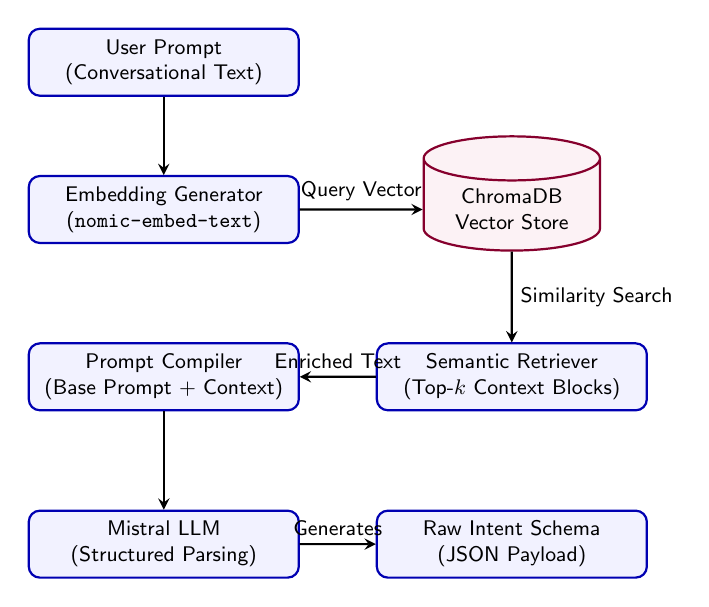
\begin{tikzpicture}[
        scale=0.85, every node/.style={transform shape, font=\sffamily\small},
        block/.style={rectangle, draw=blue!70!black, thick, fill=blue!5, text width=3.8cm, align=center, minimum height=1.0cm, rounded corners},
        db/.style={cylinder, draw=purple!70!black, thick, fill=purple!5, text width=2.4cm, align=center, minimum height=1.2cm, aspect=0.25, shape border rotate=90},
        arrow/.style={->, thick, draw=black, >=stealth}
        ]
        
        \node[block] (prompt) at (0, 0) {User Prompt\\(Conversational Text)};
        \node[block] (embed) at (0, -2.2) {Embedding Generator\\(\texttt{nomic-embed-text})};
        \node[db] (chroma) at (5.2, -2.2) {ChromaDB\\Vector Store};
        \node[block] (retrieve) at (5.2, -4.7) {Semantic Retriever\\(Top-$k$ Context Blocks)};
        \node[block] (prompteng) at (0, -4.7) {Prompt Compiler\\(Base Prompt + Context)};
        \node[block] (llm) at (0, -7.2) {Mistral LLM\\(Structured Parsing)};
        \node[block] (json) at (5.2, -7.2) {Raw Intent Schema\\(JSON Payload)};
        
        \draw[arrow] (prompt) -- (embed);
        \draw[arrow] (embed) -- node[above] {Query Vector} (chroma);
        \draw[arrow] (chroma) -- node[right] {Similarity Search} (retrieve);
        \draw[arrow] (retrieve) -- node[above] {Enriched Text} (prompteng);
        \draw[arrow] (prompteng) -- (llm);
        \draw[arrow] (llm) -- node[above] {Generates} (json);
        
    \end{tikzpicture}
    \caption{NLP and RAG Ingestion and Context Enrichment Pipeline}
    \label{fig:rag_pipeline}
\end{figure}

\subsection{Dynamic Intent Routing Engine}
The Dynamic Router (\texttt{agent/router.py}) acts as the traffic controller of the system. To minimize conversational latency and prevent API bottlenecks, the router executes a two-stage evaluation:
\begin{enumerate}
    \item \textbf{Stage-1 Direct Regex Match:} A high-performance signature check evaluating the input string against direct operational patterns (e.g., ``show policies'' or ``rollback''). If matched, it bypasses LLM computation entirely, routing the request instantly to the corresponding read wrapper.
    \item \textbf{Stage-2 Semantic LLM Classifier:} If the pattern is complex or conversational, a lightweight Mistral-small model classifies the prompt into one of five categories defined by the set $\mathcal{C}$:
    \begin{equation}
        \mathcal{C} = \{\text{READ}, \text{UPDATE}, \text{KNOWLEDGE}, \text{SECURITY\_ANALYSIS}, \text{CONVERSATIONAL}\}
    \end{equation}
    This classification set is enforced by the parsing router in \texttt{agent/router.py}, directing inputs to their respective specialized handling pipelines based on the resolved category.
\end{enumerate}

The routing separation and decision logic is visually formalized in the workflow shown in Figure~\ref{fig:routing_workflow}.

\begin{figure}[H]
    \centering
    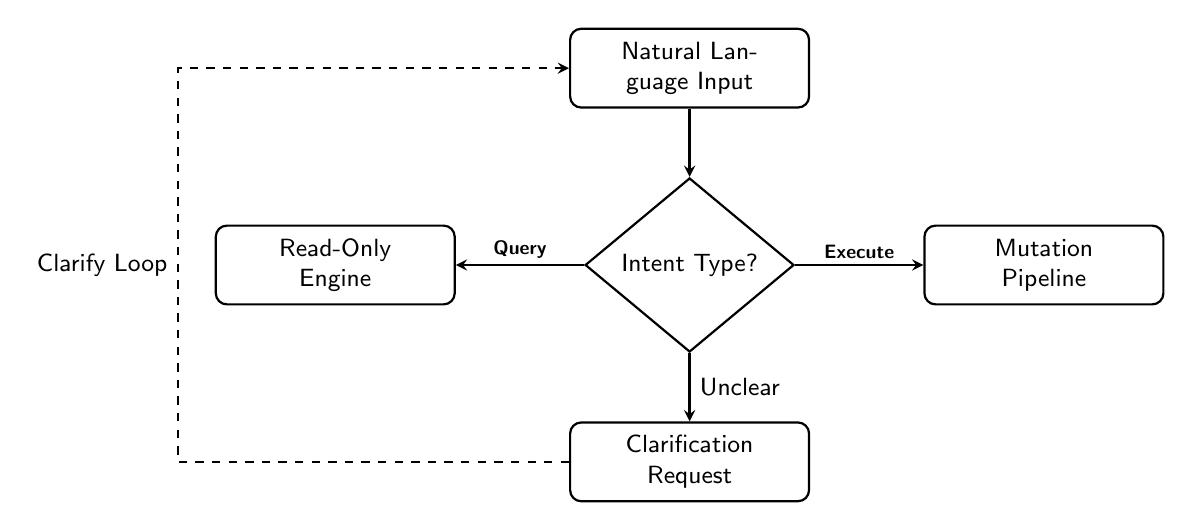
\begin{tikzpicture}[
        node distance=2.2cm,
        every node/.style={font=\sffamily\small},
        proc/.style={rectangle, draw=black, thick, fill=white, text width=2.8cm, align=center, minimum height=1.0cm, rounded corners},
        decision/.style={diamond, draw=black, thick, fill=white, text width=1.8cm, align=center, aspect=1.2},
        arrow/.style={->, thick, draw=black, >=stealth},
        badge/.style={fill=white, font=\sffamily\scriptsize\bfseries, inner sep=2pt}
        ]
        
        % Symmetrical Layout with explicit coordinates to avoid overlapping
        \node[proc] (input) at (0, 0) {Natural Language Input};
        \node[decision] (classify) at (0, -2.5) {Intent Type?};
        
        \node[proc] (read) at (-4.5, -2.5) {Read-Only\\Engine};
        \node[proc] (write) at (4.5, -2.5) {Mutation\\Pipeline};
        \node[proc] (ambig) at (0, -5.0) {Clarification\\Request};
        
        % Arrow connections with clear spacing
        \draw[arrow] (input) -- (classify);
        \draw[arrow] (classify) -- node[above, pos=0.5, badge] {Query} (read);
        \draw[arrow] (classify) -- node[above, pos=0.5, badge] {Execute} (write);
        \draw[arrow] (classify) -- node[anchor=west, pos=0.5] {Unclear} (ambig);
        
        % Spacious feedback loop going completely around the Read-Only node to avoid crossing arrows
        \draw[arrow, dashed] (ambig.west) -- (-6.5, -5.0) -- node[left, pos=0.5] {Clarify Loop} (-6.5, 0) -- (input.west);
        
    \end{tikzpicture}
    \caption{Read/Write Separation and Intent Routing Workflow}
    \label{fig:routing_workflow}
\end{figure}


\subsection{Retrieval-Augmented Generation (RAG) Enrichment}
For queries classified as \texttt{KNOWLEDGE} or requiring structural references, the system invokes the RAG pipeline:
\begin{itemize}
    \item \textbf{Embeddings Generation:} The user's raw conversational input is vectorized utilizing the local \texttt{nomic-embed-text} model via Ollama.
    \item \textbf{Vector Store Query:} The generated query vector is dispatched to a high-performance local ChromaDB instance, which indexes official FortiOS CLI manuals, best practices, and REST API documentation.
    \item \textbf{Similarity Matching:} ChromaDB executes an $L_2$ distance similarity search, returning the top-$k$ most relevant document chunks. This minimization search is computed dynamically within the vector store database according to:
    \begin{equation}
        k = \arg\min_{k} \| \vec{v}_{\text{query}} - \vec{v}_{\text{doc}_i} \|_2
    \end{equation}
    This mathematical comparison is executed by the local database engine, and the results are returned to the semantic retriever module (\texttt{rag/retriever.py}).
    \item \textbf{Prompt Assembly:} The semantic retriever extracts the text blocks, appending them directly into the Mistral system context as an immutable grounding reference, ensuring accurate, documentation-aligned answers.
\end{itemize}

\section{Translation and Execution Engine}
Once a write mutation is routed, the translation engine in \texttt{agent/nlu\_interpreter.py} prompts the Mistral model to translate the natural language command into a strictly structured \texttt{RawIntentSchema} JSON payload, defining the intent type, policy IDs, and list of changes (deltas).

\subsection{Contextual Entity Grounding Algorithm}
Because human prompts refer to firewall interfaces, address objects, and policies conversationally (e.g., ``the public server'' or ``our internal switch''), the NLU interpreter outputs raw textual variables. The entity grounder (\texttt{agent/nlu\_grounder.py}) reconciles these ambiguous references with live physical FortiOS object names.

Reconciliation is executed using a normalized Levenshtein distance ratio. Let $S_{\text{user}}$ represent the extracted string parameter and $S_{\text{device}}$ represent the actual name of a live physical firewall object. The grounding engine, implemented in the \texttt{agent/nlu\_grounder.py} module, calculates the similarity ratio as:
\begin{equation}
    \text{LevenshteinRatio}(S_{\text{user}}, S_{\text{device}}) = 1 - \frac{\text{Levenshtein}(S_{\text{user}}, S_{\text{device}})}{\max(|S_{\text{user}}|, |S_{\text{device}}|)}
\end{equation}
An entity is matched and resolved successfully to a physical object if it satisfies the threshold constraint:
\begin{equation}
    \text{LevenshteinRatio}(S_{\text{user}}, S_{\text{device}}) \ge 0.85
\end{equation}
This grounding check is programmatic logic within the \texttt{NLUObjectGrounder} class. If multiple objects satisfy this condition, the grounder flags the parameter as ambiguous, halts execution, and raises a \texttt{GroundingIssue}, which triggers the conversational clarification loop. The grounding stages of NLU extraction, live device lookup, and intent normalization are illustrated in Figure~\ref{fig:grounding_pipeline}, while the underlying programmatic logic is formalized in Algorithm~\ref{alg:grounding}.

\begin{figure}[H]
    \centering
    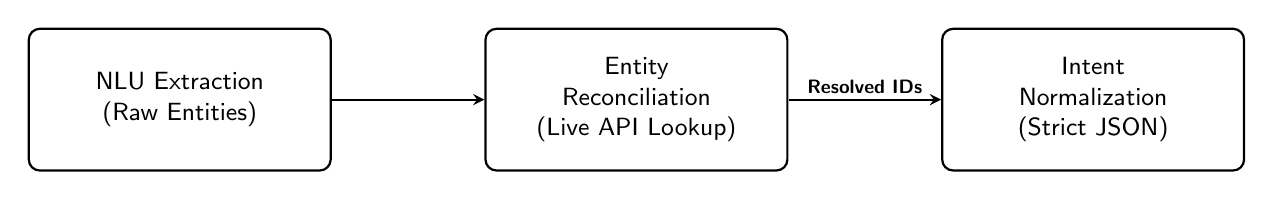
\begin{tikzpicture}[
        node distance=2.5cm,
        every node/.style={font=\sffamily\small},
        procstep/.style={rectangle, draw=black, thick, fill=white, text width=3.6cm, align=center, minimum height=1.8cm, rounded corners},
        arrow/.style={->, thick, draw=black, >=stealth},
        badge/.style={fill=white, font=\sffamily\scriptsize\bfseries, inner sep=2pt}
        ]
        
        % Symmetrical Widened Box Placements (5.8cm center-to-center distance)
        \node[procstep] (nlu) at (0, 0) {NLU Extraction\\(Raw Entities)};
        \node[procstep] (recon) at (5.8, 0) {Entity\\Reconciliation\\(Live API Lookup)};
        \node[procstep] (norm) at (11.6, 0) {Intent\\Normalization\\(Strict JSON)};
        
        % Clean Arrow Connections with Cohesive Masked Badges
        \draw[arrow] (nlu) -- (recon);
        \draw[arrow] (recon) -- node[above, pos=0.5, badge] {Resolved IDs} (norm);
        
    \end{tikzpicture}
    \caption{Entity Grounding and Live Reconciliation Pipeline}
    \label{fig:grounding_pipeline}
\end{figure}

\begin{algorithm}[H]
\caption{Dynamic Entity Grounding and Reconciliation}\label{alg:grounding}
\let\AND\undefined
\let\OR\undefined
\let\NOT\undefined
\begin{algorithmic}[1]
\REQUIRE $I_{\text{raw}}$ (Parsed Raw NLU Intent), $F_{\text{state}}$ (Live Firewall State Query)
\ENSURE $I_{\text{grounded}}$ (Grounded Target Intent) or $E_{\text{error}}$ (Grounding Ambiguity)
\STATE $O_{\text{interfaces}} \leftarrow \text{FetchLiveInterfaces}(F_{\text{state}})$
\STATE $O_{\text{addresses}} \leftarrow \text{FetchLiveAddresses}(F_{\text{state}})$
\FOR{each $E_{\text{entity}}$ in $I_{\text{raw}}.\text{entities}$}
    \STATE $S_{\text{match}} \leftarrow \emptyset$
    \FOR{each $O_{\text{obj}}$ in $O_{\text{interfaces}} \cup O_{\text{addresses}}$}
        \STATE $Score \leftarrow \text{ComputeLevenshteinRatio}(E_{\text{entity}}.\text{name}, O_{\text{obj}}.\text{name})$
        \IF{$Score \ge \text{Threshold } (0.85)$}
            \STATE $S_{\text{match}} \leftarrow S_{\text{match}} \cup \{O_{\text{obj}}\}$
        \ENDIF
    \ENDFOR
    \IF{$|S_{\text{match}}| == 1$}
        \STATE $I_{\text{grounded}}.\text{entities} \leftarrow I_{\text{grounded}}.\text{entities} \cup \{S_{\text{match}}[0]\}$
    \ELSIF{$|S_{\text{match}}| > 1$}
        \RETURN $E_{\text{error}}$ (``Ambiguous reference: multiple matches found'')
    \ELSE
        \STATE $I_{\text{grounded}}.\text{entities} \leftarrow I_{\text{grounded}}.\text{entities} \cup \text{CreateNewObjectPlaceholder}(E_{\text{entity}})$
    \ENDIF
\ENDFOR
\RETURN $I_{\text{grounded}}$
\end{algorithmic}
\end{algorithm}

\subsection{Operational Request Lifecycle}
The orchestration platform is architected as a sequential state machine. Every mutation request traverses a rigorous operational lifecycle designed to enforce security policies and maintain configuration integrity seamlessly.

\begin{table}[H]
    \centering
    \caption{Lifecycle Phases of the Operational Request Pipeline}
    \label{tab:pipeline_phases}
    \renewcommand{\arraystretch}{1.5}
    \small
    \begin{tabular}{|l|p{10.5cm}|}
        \hline
        \textbf{Pipeline Phase} & \textbf{Engineering Responsibility} \\
        \hline
        1. Ingestion & Normalizing multi-turn conversations and maintaining session context. \\
        \hline
        2. Routing & Segregating API reads, RAG queries, and infrastructure mutations. \\
        \hline
        3. Grounding & Extracting configuration parameters and reconciling network entities. \\
        \hline
        4. Validation & Deterministic syntactic and semantic checking of the proposed state. \\
        \hline
        5. HITL Review & Presenting the exact execution diff for explicit administrator authorization. \\
        \hline
        6. Pre-Execution & Capturing the live configuration baseline (snapshot) prior to modification. \\
        \hline
        7. Orchestration & Dispatching serialized REST API payloads to the target FortiGate appliance. \\
        \hline
        8. Verification & Confirming the final operational state securely matches the intended design. \\
        \hline
    \end{tabular}
\end{table}

\section{Security, Compliance, and Transactional Validation}
Once an intent is fully grounded and translated, it is routed to the deterministic validation pipeline in the control plane before reaching the firewall API.

Before any configuration payload reaches the execution layer, it is subjected to multi-tiered validation. The \textbf{Validation Engine} enforces structural integrity, ensuring that IP addresses conform to proper CIDR notations and port definitions align perfectly with standard protocols. Concurrently, the \textbf{Compliance Engine} evaluates the administrative intent against strict organizational security postures.

\begin{table}[H]
    \centering
    \caption{Multi-Tiered Validation and Security Enforcement Layers}
    \label{tab:validation_stages}
    \renewcommand{\arraystretch}{1.5}
    \small
    \begin{tabular}{|l|l|p{6.5cm}|}
        \hline
        \textbf{Validation Tier} & \textbf{Mechanism} & \textbf{Operational Focus} \\
        \hline
        \textbf{Syntactic Layer} & Regex \& Type Checking & Validating IP formats, protocol numbers, and API schema adherence. \\
        \hline
        \textbf{Semantic Layer} & Entity Reconciliation & Ensuring requested objects and policy IDs exist dynamically on the firewall. \\
        \hline
        \textbf{Compliance Layer} & Policy Ruleset Evaluation & Proactively preventing least-privilege violations (e.g., blocking 0.0.0.0/0 on SSH). \\
        \hline
    \end{tabular}
\end{table}


\subsection{Proactive Compliance and Safety Engine}
The \texttt{agent/compliance.py} module implements a rule-based validation engine that enforces security best practices, protecting the enterprise perimeter from accidental administrative misconfigurations. 

We represent a planned firewall policy mutation as $P$, defined by:
\begin{equation}
    P = \langle S_{\text{addr}}, D_{\text{addr}}, Src_{\text{intf}}, Dst_{\text{intf}}, Serv, Act \rangle
\end{equation}
Where $S_{\text{addr}}$ is the source address, $D_{\text{addr}}$ is the destination address, $Src_{\text{intf}}$ is the source interface, $Dst_{\text{intf}}$ is the destination interface, $Serv$ is the list of permitted services, and $Act \in \{\text{accept}, \text{deny}\}$ is the policy action. These compliance filters are implemented as deterministic check methods inside the \texttt{agent/compliance.py} module, executing static validation rules before any REST API update is prepared.

The compliance engine enforces three core validation safety checks:
\begin{enumerate}
    \item \textbf{Implicit Deny Enforcement (Any-to-Any Accept Prevention):}
    If the planned policy permits traffic, it must not apply to global wildcards on both interfaces simultaneously:
    \begin{equation}
        P_{\text{valid}} \implies \neg \big( (Act = \text{accept}) \land (Src_{\text{intf}} = \text{"any"}) \land (Dst_{\text{intf}} = \text{"any"}) \big)
    \end{equation}
    Violations of this rule trigger an immediate safety block within the compliance validator, throwing an exception and halting the orchestrator.
    
    \item \textbf{Insecure Interface Protocol Blocking:}
    Let $I_{\text{protocols}}$ represent the administrative access protocols enabled on a target management interface. The system must prevent binding insecure legacy protocols:
    \begin{equation}
        Access_{\text{valid}} \implies (I_{\text{protocols}} \cap \{\text{"HTTP"}, \text{"TELNET"}\} = \emptyset)
    \end{equation}
    If an operator attempts to enable these protocols on any interface, the validation engine rejects the transaction.
    
    \item \textbf{Insecure Port Public Exposure Prevention:}
    Let $Serv_{\text{ports}}$ represent the TCP/UDP ports mapped to a policy. If a policy bridges a public interface (WAN) to an internal subnet, it must not expose highly vulnerable legacy services (such as SMB or RDP):
    \begin{equation}
        Exposure_{\text{valid}} \implies \Big( Src_{\text{intf}} \in \text{WAN} \implies (Serv_{\text{ports}} \cap \{137, 138, 139, 445, 3389\} = \emptyset) \Big)
    \end{equation}
\end{enumerate}

\subsection{Session Context and Conceptual State Transitions}
To maintain state consistency during multi-turn interactions (such as clarifications or awaiting administrative confirmation), the orchestrator manages a conceptual session lifecycle. Rather than relying on a strict, hardware-bound finite state machine (FSM) implementation, this state machine represents the logical, session-driven context transitions managed dynamically by the \texttt{AgentSession} class. These conceptual states and their permitted transitions are illustrated in Figure~\ref{fig:state_machine}.

To enable robust interaction, the system supports clarification continuity and partial intent persistence. When the user provides an incomplete or ambiguous intent (e.g., "Allow HTTP access" without specifying a destination address), the system transitions to the \texttt{CLARIFY} state. The partial parameters are persisted in memory within the \texttt{SessionContext} class (implemented in \texttt{agent/session\_context.py}). Upon the next user turn, the input is merged with the existing context and re-grounded, ensuring deterministic multi-turn validation without forcing the administrator to restart the command sequence.

\begin{figure}[H]
    \centering
    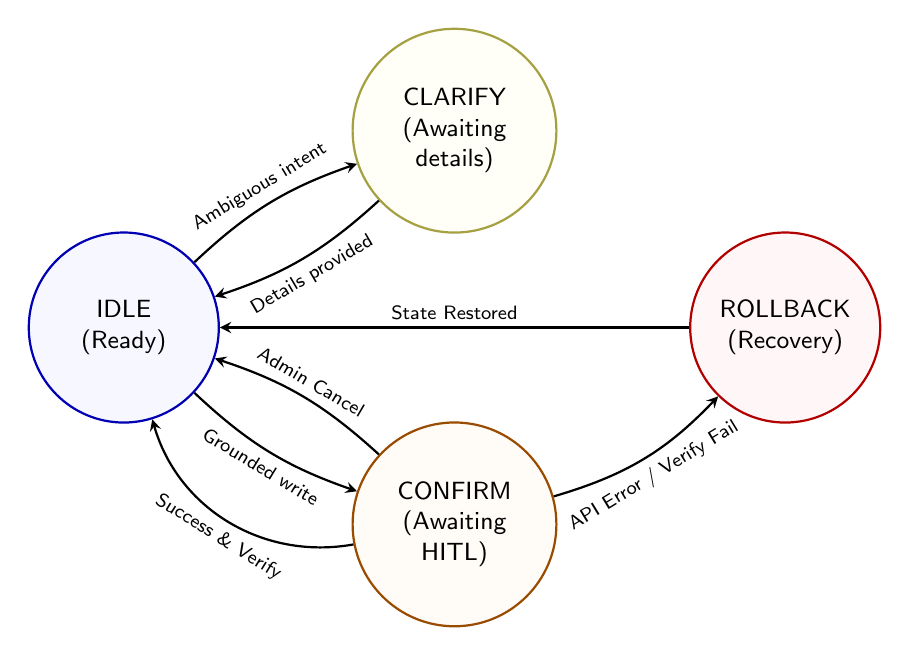
\begin{tikzpicture}[
        node distance=3.0cm,
        every node/.style={font=\sffamily\small},
        stateidle/.style={circle, draw=blue!70!black, thick, fill=blue!3, text width=2.0cm, align=center, minimum height=2.0cm},
        stateclarify/.style={circle, draw=yellow!60!black, thick, fill=yellow!3, text width=2.0cm, align=center, minimum height=2.0cm},
        stateconfirm/.style={circle, draw=orange!60!black, thick, fill=orange!3, text width=2.0cm, align=center, minimum height=2.0cm},
        staterollback/.style={circle, draw=red!70!black, thick, fill=red!3, text width=2.0cm, align=center, minimum height=2.0cm},
        arrow/.style={->, thick, draw=black, >=stealth}
        ]
        
        \node[stateidle] (idle) at (0, 0) {IDLE\\(Ready)};
        \node[stateclarify] (clarify) at (4.2, 2.5) {CLARIFY\\(Awaiting\\details)};
        \node[stateconfirm] (confirm) at (4.2, -2.5) {CONFIRM\\(Awaiting\\HITL)};
        \node[staterollback] (rollback) at (8.4, 0) {ROLLBACK\\(Recovery)};
        
        \draw[arrow] (idle) to[bend left=12] node[above, sloped, font=\sffamily\scriptsize] {Ambiguous intent} (clarify);
        \draw[arrow] (clarify) to[bend left=12] node[below, sloped, font=\sffamily\scriptsize] {Details provided} (idle);
        
        \draw[arrow] (idle) to[bend right=12] node[below, sloped, font=\sffamily\scriptsize] {Grounded write} (confirm);
        \draw[arrow] (confirm) to[bend right=12] node[above, sloped, font=\sffamily\scriptsize] {Admin Cancel} (idle);
        
        \draw[arrow] (confirm) to[bend right=15] node[below, sloped, font=\sffamily\scriptsize] {API Error / Verify Fail} (rollback);
        \draw[arrow] (confirm) to[bend left=42] node[below, sloped, font=\sffamily\scriptsize] {Success \& Verify} (idle);
        \draw[arrow] (rollback) to node[above, font=\sffamily\scriptsize, fill=white, inner sep=2.5pt] {State Restored} (idle);
        
    \end{tikzpicture}
    \caption{State Transition Diagram for multi-turn Administrator Sessions}
    \label{fig:state_machine}
\end{figure}

This session lifecycle manages the safety invariant that the session context cannot transition from \texttt{IDLE} directly to a device mutation without systematically transitioning through the validated and operator-reviewed \texttt{CONFIRM} state.

\subsection{Lifecycle Management \& Transactional Recovery}
To maintain database and network state alignment, the orchestrator encapsulates mutations within a \textbf{Transactional Execution Loop}, implementing a strict try-verify-rollback strategy:
\begin{enumerate}
    \item \textbf{Pre-Mutation Snapshot:} Captures the target configuration parameters (e.g., current ruleset ordering, specific policy parameters) and stores them in a localized stack buffer managed by the \texttt{SnapshotStore} class (\texttt{agent/snapshot.py}).
    \item \textbf{Atomic Execution:} Applies the API changes directly to the FortiOS REST endpoint. The REST client enforces a strict 5-second timeout window; connections exceeding this threshold are aborted to prevent session hanging.
    \item \textbf{Active State Verification:} Immediately issues a post-write query to read back the active state. If the returned state does not match the expected state delta, or if a connection loss occurs (monitored by HTTP heartbeat pings), the system marks the transaction as failed.
    \item \textbf{Inverse Rollback:} Restores the pre-mutation parameters captured in the snapshot, reverting the firewall to its last known stable state.
\end{enumerate}

\subsubsection{Operational Recovery Boundaries and Limitations}
While the transactional loop mitigates deployment risks, physical networking constraints introduce specific operational boundaries:
\begin{itemize}
    \item \textbf{Rollback Connectivity Dependency}: If a configuration mutation inadvertently severs the physical network interface or administrative IP access used by the orchestrator (e.g., changing the management gateway to an unreachable route), the orchestrator will be unable to transmit the inverse rollback payload. In this scenario, the system flags a high-priority alarm on the console and halts, requiring manual physical or out-of-band console recovery.
    \item \textbf{State Persistence Boundaries}: The snapshot buffer writes state directly to local disk (\texttt{logs/snapshots.json}) prior to any mutation. This guarantees that even if the management client or container crashes during execution, the rollback state survives and can be explicitly restored upon system recovery.
\end{itemize}

This fail-safe validation and rollback process is visually modeled in Figure~\ref{fig:verification_workflow}.

\begin{figure}[H]
    \centering
    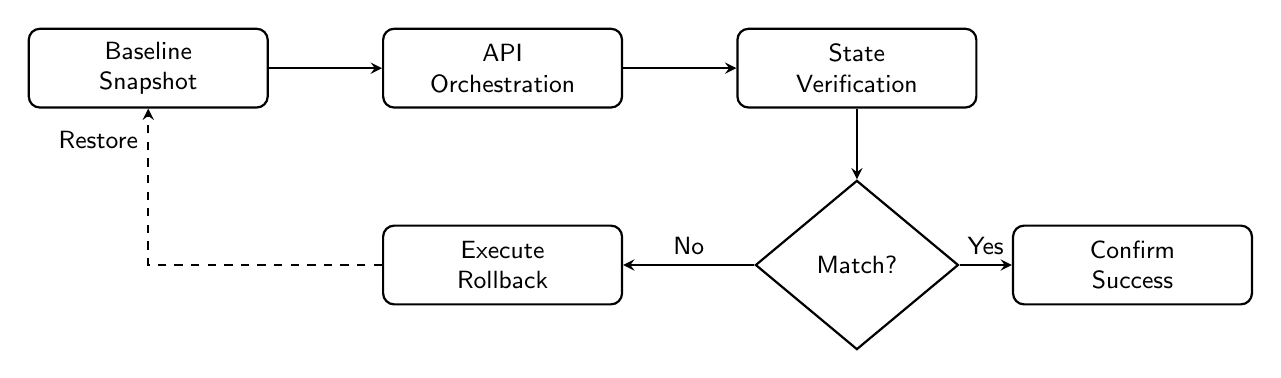
\begin{tikzpicture}[
        node distance=2.2cm,
        every node/.style={font=\sffamily\small},
        action/.style={rectangle, draw=black, thick, fill=white, text width=2.8cm, align=center, minimum height=1.0cm, rounded corners},
        decision/.style={diamond, draw=black, thick, fill=white, text width=1.8cm, align=center, aspect=1.2},
        arrow/.style={->, thick, draw=black, >=stealth}
        ]
        
        \node[action] (snap) at (0, 0) {Baseline\\Snapshot};
        \node[action] (exec) at (4.5, 0) {API\\Orchestration};
        \node[action] (ver) at (9.0, 0) {State\\Verification};
        \node[decision] (check) at (9.0, -2.5) {Match?};
        
        \node[action] (rollback) at (4.5, -2.5) {Execute\\Rollback};
        \node[action] (commit) at (12.5, -2.5) {Confirm\\Success};
        
        \draw[arrow] (snap) -- (exec);
        \draw[arrow] (exec) -- (ver);
        \draw[arrow] (ver) -- (check);
        \draw[arrow] (check) -- node[above] {No} (rollback);
        \draw[arrow] (check) -- node[above] {Yes} (commit);
        
        % Horizontal-vertical restore line routing back cleanly to Baseline Snapshot bottom edge
        \draw[arrow, dashed] (rollback.west) -- (0, -2.5) -- node[left, pos=0.8] {Restore} (snap.south);
        
    \end{tikzpicture}
    \caption{Transactional Verification and Lifecycle Management Workflow}
    \label{fig:verification_workflow}
\end{figure}

\subsection{Structured Audit and Integrity Logging}
To ensure all configuration changes are completely auditable and detectable against local tampering, the logging component writes transaction logs using a structured rolling hash chain. Each transaction record $T_n$ is chained to the preceding record $T_{n-1}$ by computing:
\begin{equation}
    H(T_n) = \text{SHA-256}\big(T_n.\text{payload} \mathbin{\Vert} H(T_{n-1})\big)
\end{equation}
This validation formula, implemented in our audit logging wrapper, ensures that any unauthorized manual edits to the local log files in \texttt{logs/audit.jsonl} immediately invalidate the sequential hash sequence. It provides local integrity verification for audit trails rather than absolute cryptographic non-repudiation or blockchain-grade guarantees.

\section{UML Use Case and Structural Modeling}
To map the active interfaces and object relationships that control the transactional pipeline, we provide formal Unified Modeling Language (UML) notations of the system.

The interaction boundaries between the system operator (network administrator), the hybrid orchestration agent, and the physical FortiGate firewall are modeled in the global Use Case diagram shown in Figure~\ref{fig:uml_use_case}.

\begin{figure}[H]
    \centering
    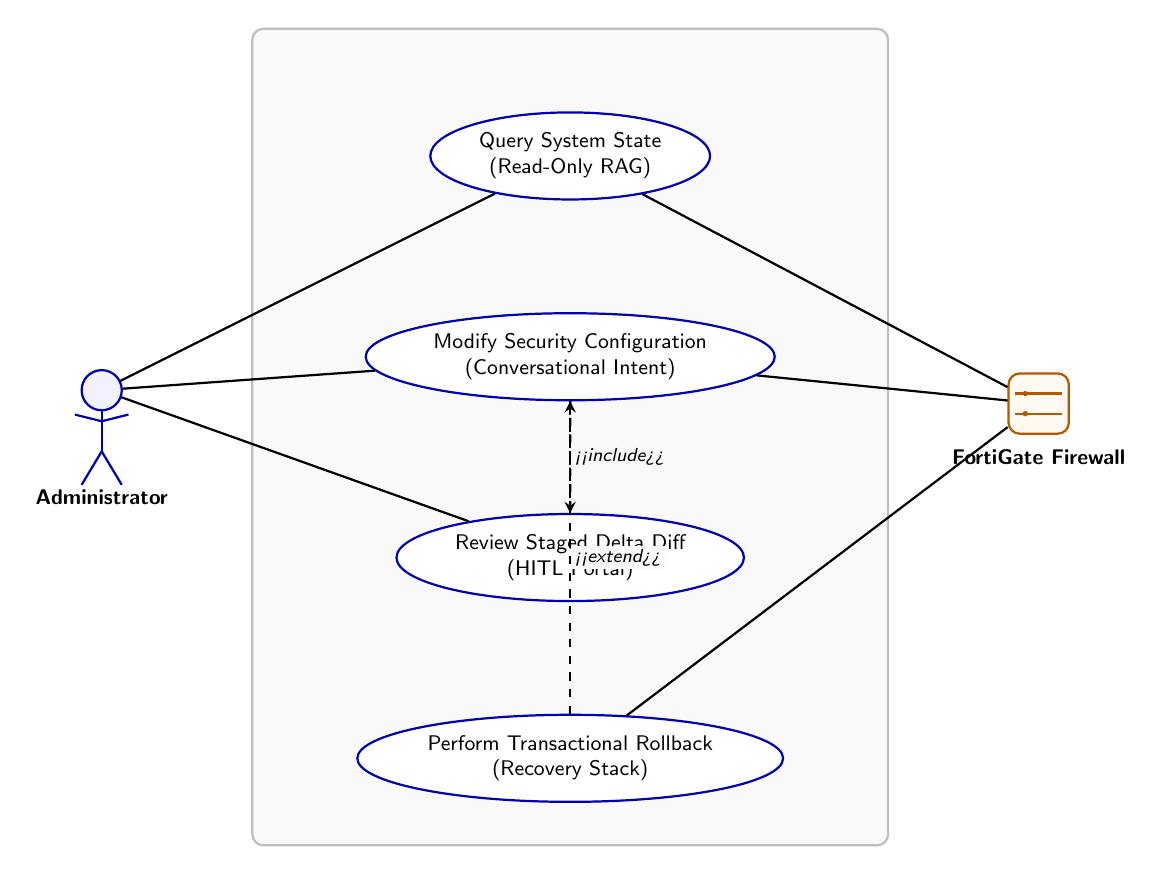
\begin{tikzpicture}[
        scale=0.85, every node/.style={transform shape},
        actorhead/.style={draw=blue!70!black, thick, circle, minimum size=0.6cm, fill=blue!5},
        firewallbox/.style={draw=orange!70!black, thick, rectangle, minimum width=0.9cm, minimum height=0.9cm, rounded corners, fill=orange!5},
        usecase/.style={draw=blue!70!black, thick, ellipse, minimum width=3.4cm, minimum height=1.0cm, align=center, fill=white, font=\sffamily\small},
        systembox/.style={draw=gray!50, thick, rectangle, minimum width=9.5cm, minimum height=12.2cm, fill=gray!5, rounded corners},
        arrow/.style={-, thick, draw=black},
        include/.style={->, dashed, thick, draw=black, >=stealth, font=\sffamily\scriptsize}
        ]
        
        % Boundaries \& System Container
        \node[systembox] (sys) at (5.0, -5.7) {};
        %\node[font=\sffamily\small\bfseries\color{gray!80}] at (5.0, -0.0) {FortiGate Orchestrator Boundary};
        
        % Operator Actor (Stick Figure Head)
        \node[actorhead] (admin) at (-2.0, -5.0) {};
        % Stick Figure Body \& Limbs
        \draw[thick, draw=blue!70!black] (admin.south) -- ++(0, -0.6) coordinate (torso);
        \draw[thick, draw=blue!70!black] (torso) -- ++(-0.3, -0.5);
        \draw[thick, draw=blue!70!black] (torso) -- ++(0.3, -0.5);
        \draw[thick, draw=blue!70!black] (admin.south) ++(0, -0.15) -- ++(-0.4, 0.1);
        \draw[thick, draw=blue!70!black] (admin.south) ++(0, -0.15) -- ++(0.4, 0.1);
        \node[font=\sffamily\small\bfseries] at (-2.0, -6.6) {Administrator};
        
        % Firewall Device Actor (Server Rack Representation)
        \node[firewallbox] (fw) at (12.0, -5.2) {};
        \draw[thick, draw=orange!70!black] (11.65, -5.05) -- (12.35, -5.05);
        \draw[thick, draw=orange!70!black] (11.65, -5.35) -- (12.35, -5.35);
        \fill[orange!70!black] (11.8, -5.05) circle (0.04cm);
        \fill[orange!70!black] (11.8, -5.35) circle (0.04cm);
        \node[font=\sffamily\small\bfseries] at (12.0, -6.0) {FortiGate Firewall};
        
        % Use Cases inside boundary
        \node[usecase] (uc1) at (5.0, -1.5) {Query System State\\(Read-Only RAG)};
        \node[usecase] (uc2) at (5.0, -4.5) {Modify Security Configuration\\(Conversational Intent)};
        \node[usecase] (uc3) at (5.0, -7.5) {Review Staged Delta Diff\\(HITL Portal)};
        \node[usecase] (uc4) at (5.0, -10.5) {Perform Transactional Rollback\\(Recovery Stack)};
        
        % Administrative Links (connected to head node)
        \draw[arrow] (admin) -- (uc1);
        \draw[arrow] (admin) -- (uc2);
        \draw[arrow] (admin) -- (uc3);
        
        % Firewall Links (connected to firewall node)
        \draw[arrow] (uc1) -- (fw);
        \draw[arrow] (uc2) -- (fw);
        \draw[arrow] (uc4) -- (fw);
        
        % Dependencies (includes \& extends)
        \draw[include] (uc2) -- node[right, fill=gray!5, inner sep=1.5pt] {\footnotesize\textit{<<include>>}} (uc3);
        \draw[include] (uc4) -- node[right, fill=gray!5, inner sep=1.5pt] {\footnotesize\textit{<<extend>>}} (uc2);
        
    \end{tikzpicture}
    \caption{UML Use Case Diagram representing Operator Interactions and System Boundaries}
    \label{fig:uml_use_case}
\end{figure}

The structural design of the Python backend is modeled in the UML Class Diagram shown in Figure~\ref{fig:uml_class_diagram}. This diagram illustrates the properties, methods, and relationships of the active modules.

\begin{figure}[H]
    \centering
    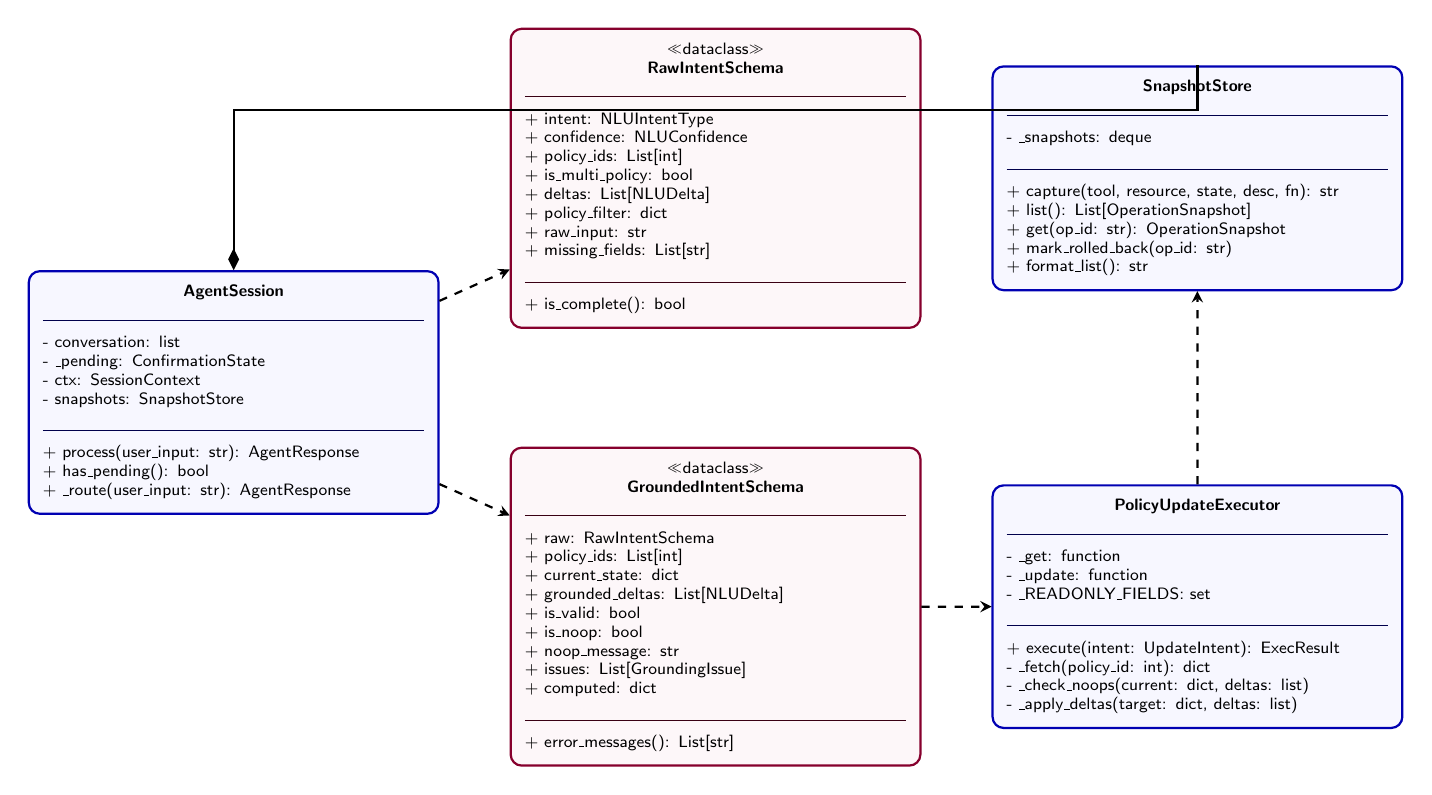
\begin{tikzpicture}[
        scale=0.85, every node/.style={transform shape},
        classbox/.style={rectangle, draw=blue!70!black, thick, fill=blue!3, text width=5.7cm, align=left, rounded corners, font=\sffamily\scriptsize, inner sep=6pt},
        dataclassbox/.style={rectangle, draw=purple!70!black, thick, fill=purple!3, text width=5.7cm, align=left, rounded corners, font=\sffamily\scriptsize, inner sep=6pt},
        arrow/.style={->, thick, draw=black, >=stealth},
        dependency/.style={->, thick, dashed, draw=black, >=stealth},
        composition/.style={{Diamond[black]}-, thick, draw=black, >=stealth}
        ]
        
        % Class 1: AgentSession
        \node[classbox] (session) at (0, 0) {
            {\centering\textbf{AgentSession}\par}\vspace{0.08cm}
            {\color{blue!30!black}\rule{\linewidth}{0.4pt}}\\[0.12cm]
            - conversation: list\\
            - \_pending: ConfirmationState\\
            - ctx: SessionContext\\
            - snapshots: SnapshotStore\\[0.12cm]
            {\color{blue!30!black}\rule{\linewidth}{0.4pt}}\\[0.12cm]
            + process(user\_input: str): AgentResponse\\
            + has\_pending(): bool\\
            + \_route(user\_input: str): AgentResponse
        };
        
        % Class 2: RawIntentSchema
        \node[dataclassbox] (nlu) at (7.2, 3.2) {
            {\centering\guillemotleft dataclass\guillemotright\\ \textbf{RawIntentSchema}\par}\vspace{0.08cm}
            {\color{purple!30!black}\rule{\linewidth}{0.4pt}}\\[0.12cm]
            + intent: NLUIntentType\\
            + confidence: NLUConfidence\\
            + policy\_ids: List[int]\\
            + is\_multi\_policy: bool\\
            + deltas: List[NLUDelta]\\
            + policy\_filter: dict\\
            + raw\_input: str\\
            + missing\_fields: List[str]\\[0.12cm]
            {\color{purple!30!black}\rule{\linewidth}{0.4pt}}\\[0.12cm]
            + is\_complete(): bool
        };
        
        % Class 3: GroundedIntentSchema
        \node[dataclassbox] (grounder) at (7.2, -3.2) {
            {\centering\guillemotleft dataclass\guillemotright\\ \textbf{GroundedIntentSchema}\par}\vspace{0.08cm}
            {\color{purple!30!black}\rule{\linewidth}{0.4pt}}\\[0.12cm]
            + raw: RawIntentSchema\\
            + policy\_ids: List[int]\\
            + current\_state: dict\\
            + grounded\_deltas: List[NLUDelta]\\
            + is\_valid: bool\\
            + is\_noop: bool\\
            + noop\_message: str\\
            + issues: List[GroundingIssue]\\
            + computed: dict\\[0.12cm]
            {\color{purple!30!black}\rule{\linewidth}{0.4pt}}\\[0.12cm]
            + error\_messages(): List[str]
        };
        
        % Class 4: SnapshotStore
        \node[classbox] (snapshot) at (14.4, 3.2) {
            {\centering\textbf{SnapshotStore}\par}\vspace{0.08cm}
            {\color{blue!30!black}\rule{\linewidth}{0.4pt}}\\[0.12cm]
            - \_snapshots: deque\\[0.12cm]
            {\color{blue!30!black}\rule{\linewidth}{0.4pt}}\\[0.12cm]
            + capture(tool, resource, state, desc, fn): str\\
            + list(): List[OperationSnapshot]\\
            + get(op\_id: str): OperationSnapshot\\
            + mark\_rolled\_back(op\_id: str)\\
            + format\_list(): str
        };
        
        % Class 5: PolicyUpdateExecutor
        \node[classbox] (executor) at (14.4, -3.2) {
            {\centering\textbf{PolicyUpdateExecutor}\par}\vspace{0.08cm}
            {\color{blue!30!black}\rule{\linewidth}{0.4pt}}\\[0.12cm]
            - \_get: function\\
            - \_update: function\\
            - \_READONLY\_FIELDS: set\\[0.12cm]
            {\color{blue!30!black}\rule{\linewidth}{0.4pt}}\\[0.12cm]
            + execute(intent: UpdateIntent): ExecResult\\
            - \_fetch(policy\_id: int): dict\\
            - \_check\_noops(current: dict, deltas: list)\\
            - \_apply\_deltas(target: dict, deltas: list)
        };
        
        % Relationships
        \draw[dependency] (session) -- (nlu);
        \draw[dependency] (session) -- (grounder);
        \draw[dependency] (grounder) -- (executor);
        \draw[dependency] (executor) -- (snapshot);
        \draw[composition] (session.north) -- ++(0, 2.4) -| (snapshot.north);
        
    \end{tikzpicture}
    \caption{UML Class Diagram representing structural relationships of Python Backend Classes}
    \label{fig:uml_class_diagram}
\end{figure}

The `AgentSession` context class acts as the central coordinator, orchestrating transitions between the conversational NLU layers and the deterministic components. The dynamic NLU parsing yields `RawIntentSchema` instances, which are immediately directed to the grounding engine to produce verified `GroundedIntentSchema` structures. Finally, mutations are managed by the `PolicyUpdateExecutor` coupled with the transactional recovery capabilities of the `SnapshotStore` to ensure fail-safe operation on the physical firewall appliance.

\section{Chapter Conclusion}
This chapter has detailed the architectural design, ingestion pipelines, and structural specifications of the hybrid network orchestration prototype. By segregating the system into a probabilistic interpretation plane and a deterministic control plane, we enforce a strict trust boundary. We have modeled the NLP \& RAG enrichment stages, established functional diagrams using UML Use Cases, defined the detailed software components using class models, and mathematically formulated the safety gates that enforce corporate security postures. These designs establish a highly precise, verifiable blueprint for secure network automation.

\chapter{Implementation, Testing, and Validation}


\section{Introduction}
The implementation, testing, and validation phase constitutes the practical realization of the Trust Boundary Architecture proposed in Chapter 3. While Chapter 3 established the conceptual and structural design of the hybrid FortiGate AI Agent, this chapter shifts the focus to engineering substance: the actual implemented Python codebase, its measurable technical metrics, the precise algorithms governing the critical safety mechanisms, and a rigorous empirical validation campaign structured as a series of architectural proofs.

This chapter is organized as follows. Section~\ref{sec:env} describes the hardware and software environment used during development and validation. Section~\ref{sec:implementation} provides a technical audit of the implemented codebase, covering directory structure, file metrics, and a detailed description of each core software component. Section~\ref{sec:listings} presents the actual implemented source code for the most architecturally significant algorithms. Section~\ref{sec:validation} contains the structured validation campaign, framing each test as an \emph{architectural proof} that empirically demonstrates a specific safety claim of the Trust Boundary Architecture. Section~\ref{sec:ui} demonstrates the Streamlit Security Operations Center interface and its integration with the agent backend. Section~\ref{sec:docker} details the containerized deployment architecture. Finally, Section~\ref{sec:limits} acknowledges the architectural limitations of the current implementation and Section~\ref{sec:future} outlines future directions.

% -------------------------------------------------------------
\section{Development and Testing Environment}
\label{sec:env}

To validate the safety guarantees and performance parameters of the FortiGate AI Agent, a dedicated local engineering environment was established. Table~\ref{tab:env_specs} summarizes the full environment specification.

\begin{table}[htpb]
\centering
\small
\begin{tabular}{|l|p{9cm}|}
\hline
\textbf{Component} & \textbf{Specification} \\ \hline
\textbf{CPU} & AMD Ryzen 7 (8 cores, 16 threads) \\ \hline
\textbf{Memory} & 32 GB DDR4 RAM \\ \hline
\textbf{GPU} & NVIDIA GeForce RTX 4060 (8 GB VRAM) \\ \hline
\textbf{Operating System} & Windows 11 with WSL2 backend for containerized services \\ \hline
\textbf{Firewall Appliance} & Fortinet FortiGate VM running FortiOS v7.0.5 (local hypervisor). REST API exposed over HTTPS on the management interface at \texttt{192.168.1.134}. \\ \hline
\textbf{Runtime Language} & Python 3.11 (orchestration, NLU, validation, and UI layers) \\ \hline
\textbf{NLU Model} & \texttt{mistral-small-latest} via Mistral API. Temperature locked to $T=0.0$ for full reproducibility. Output constrained to strict JSON schema. \\ \hline
\textbf{Vector Database} & ChromaDB v0.4 (local persistent store for RAG pipeline) \\ \hline
\textbf{UI Framework} & Streamlit v1.28 (dark-mode SOC-style chat dashboard) \\ \hline
\textbf{HTTP Client} & \texttt{httpx} v0.25 (async-capable REST communication with FortiGate API) \\ \hline
\textbf{Test Framework} & \texttt{pytest} v7.4 (unit and integration test automation) \\ \hline
\end{tabular}
\caption{Environment Specifications}
\label{tab:env_specs}
\end{table}

The choice of \texttt{mistral-small-latest} is deliberate. As established in Chapter 2, the role of the LLM in this architecture is strictly confined to \emph{intent parsing}—transforming unstructured natural language into a raw JSON schema. Setting temperature to $T=0.0$ eliminates stochastic generation, making the NLU output deterministic for identical inputs during validation runs. This reproducibility is essential for the empirical testing methodology applied in Section~\ref{sec:validation}.

% -------------------------------------------------------------
\section{System Implementation and Technical Audit}
\label{sec:implementation}

\subsection{Codebase Directory Structure and File Metrics}
\label{subsec:metrics}

The project codebase is strictly partitioned to enforce the trust boundary defined in Chapter 3. All probabilistic components (NLU interpreting and RAG retrieval) are isolated from all deterministic components (validation, compliance, snapshot, and REST API execution). Table~\ref{tab:codebase_metrics} audits the implemented files, detailing their relative path, measured line count, and primary architectural responsibility.

\begin{longtable}{|l|c|p{7.5cm}|}
\caption{Codebase Structure and Metrics}
\label{tab:codebase_metrics} \\
\hline
\textbf{File Relative Path} & \textbf{Lines} & \textbf{Architectural Responsibility} \\ \hline
\endfirsthead

\multicolumn{3}{c}%
{{\bfseries \tablename\ \thetable{} -- continued from previous page}} \\
\hline
\textbf{File Relative Path} & \textbf{Lines} & \textbf{Architectural Responsibility} \\ \hline
\endhead

\hline \multicolumn{3}{|r|}{{Continued on next page}} \\ \hline
\endfoot

\hline
\endlastfoot

\texttt{agent/core.py} & 2,417 & Master session orchestrator. Coordinates routing classification, session state machine transitions, grounding, compliance pre-checks, HITL confirmation, and post-execution verification. \\ \hline
\texttt{agent/compliance.py} & 450 & Proactive deterministic compliance engine. Evaluates proposed configuration changes against a static ruleset (POL-001 through POL-005, INTF-001) before any API call is dispatched. \\ \hline
\texttt{agent/nlu\_interpreter.py} & 765 & NLU layer. Constructs and dispatches Mistral API prompts, then parses and normalizes the returned JSON output via markdown-fence extraction and structural normalization. \\ \hline
\texttt{agent/nlu\_grounder.py} & 932 & Contextual grounding engine. Resolves raw NLU-extracted entity names and IDs against live FortiGate API state using exact matching and Levenshtein distance scoring. \\ \hline
\texttt{agent/nlu\_schema.py} & 112 & Shared data structures. Declares \texttt{RawIntentSchema}, \texttt{GroundedIntentSchema}, \texttt{NLUDelta}, and \texttt{GroundingIssue} dataclasses. \\ \hline
\texttt{agent/router.py} & 598 & Two-stage intent router. Stage 1 applies deterministic regex filters for high-confidence patterns. Stage 2 dispatches ambiguous inputs to the LLM-based semantic classifier. \\ \hline
\texttt{agent/session\_context.py} & 401 & Short-term conversational memory manager. Tracks active entity focus, sliding-window entity stack, and performs pronoun resolution and clarification-state management. \\ \hline
\texttt{agent/snapshot.py} & 544 & Transactional safety layer. Captures pre-mutation resource state via HTTP GET, persists snapshots to disk, and executes PUT-based rollback restoration. \\ \hline
\texttt{agent/validator.py} & 578 & Structural input validator. Verifies IP address formats, subnet validity, CIDR legality, port range correctness, and interface lockout hazard detection. \\ \hline
\texttt{agent/tools.py} & 1,480 & FortiGate REST API wrapper. Encapsulates all GET, POST, PUT, and DELETE API calls across policy, address, interface, and system resource endpoints. \\ \hline
\texttt{audit/logger.py} & 156 & Cryptographic audit logger. Writes append-only JSONL entries with rolling SHA-256 hash chains, creating a tamper-evident ledger. \\ \hline
\texttt{audit/report.py} & 101 & Audit report and integrity verifier. Re-computes hash chain and flags any deleted, altered, or reordered log entries. \\ \hline
\texttt{streamlit\_app.py} & 210 & SOC-style Streamlit dashboard. Renders conversation UI, live resource meters, FortiGate connection indicator, and delta diff confirmations. \\ \hline
\end{longtable}

The total codebase spans approximately \textbf{8,744 lines} of production Python, distributed across 13 primary modules. This figure excludes test suites, documentation files, and Docker configuration. The largest module is \texttt{agent/core.py} at 2,417 lines, reflecting the architectural complexity of the session state machine, which must coordinate between all other modules while maintaining full transactional integrity. The second largest is \texttt{agent/tools.py} at 1,480 lines, representing the comprehensive coverage of the FortiGate v7.0.5 REST API surface.

\subsection{Natural Language Understanding and Intent Extraction}
\label{subsec:nlu}

The NLU interpreter module (\texttt{agent/nlu\_interpreter.py}) serves as the sole and tightly controlled interface between the user's natural language input and the deterministic processing pipeline. It is designed with a fundamental engineering constraint: \emph{the LLM output is never trusted directly}.

The module operates in three sequential stages:

\begin{enumerate}
    \item \textbf{Prompt Construction:} The interpreter builds a structured prompt that embeds the user's message alongside the current FortiGate device context (available policies, interfaces, address objects, and service groups fetched via live REST API). Injecting live context is a critical security measure: it bounds the LLM's operational vocabulary to actually existing objects, reducing the probability of hallucinated references.
    \item \textbf{JSON Extraction (\texttt{\_extract\_json()}):} The raw API response is not trusted to be valid JSON. The extraction algorithm first searches for markdown code fences (\texttt{```json ... ```}) using a regular expression scan, since the Mistral model wraps its output in such blocks. If a fence is found, the content is extracted. If no fence exists, the algorithm attempts to locate the first \texttt{\{} and last \texttt{\}} characters to carve out the JSON object. This dual-path extraction is necessary for robustness across LLM output variations.
    \item \textbf{Structural Normalization (\texttt{\_normalize\_dict()}):} The extracted JSON is mapped through a normalization table that handles case variations, French synonyms (``activer'' $\to$ \texttt{enable}, ``désactiver'' $\to$ \texttt{disable}), and field aliases (\texttt{src} $\to$ \texttt{srcaddr}). After normalization, the dict is deserialized into the strongly-typed \texttt{RawIntentSchema} dataclass. Any field mismatch or missing required key raises a \texttt{NLUParseError}, which is caught by the orchestrator and surfaced to the user as a clarification request.
\end{enumerate}

\subsection{Contextual Entity Grounding and Normalization}
\label{subsec:grounding}

The grounding engine (\texttt{agent/nlu\_grounder.py}) constitutes the primary architectural barrier against LLM hallucinations. Once the NLU layer produces a \texttt{RawIntentSchema}, the grounding engine validates every extracted entity (policy IDs, policy names, interface names, address group names) against the actual, live state of the FortiGate appliance.

The grounding algorithm proceeds as follows for a policy reference:

\begin{enumerate}
    \item \textbf{API Query:} A direct HTTP GET request is dispatched to
    \texttt{/api/v2/cmdb/firewall/\allowbreak{}policy/<id>}.
    A 404 response conclusively proves the entity does not exist.
    \item \textbf{Name Resolution (Fuzzy Matching):} If a name is provided instead of an ID, the engine fetches the full policy list via \texttt{/api/v2/cmdb/firewall/policy/} and scores each candidate against the extracted name using Levenshtein edit distance~\cite{navarro2001guided}. A match is only accepted if the edit distance is below a defined threshold \emph{and} the normalized candidate names are unique (no ambiguous matches).
    \item \textbf{Issue Registration:} Any failed resolution (404 response, no match found, or multiple matches above threshold) is recorded as a \texttt{GroundingIssue} and appended to the \texttt{GroundedIntentSchema.issues} list. The orchestrator inspects this list after grounding and blocks execution if any unresolved issue of \texttt{kind=``not\_found''} or \texttt{kind=``ambiguous''} is present.
\end{enumerate}

Critically, the grounding engine \emph{never raises exceptions to the caller}. Its contract is to always return a fully populated \texttt{GroundedIntentSchema}, with the \texttt{is\_valid} flag set to \texttt{False} if any blocking issue was encountered. This guarantees that the orchestrator's control flow remains deterministic even in the face of API failures or malformed LLM output.

\subsection{Deterministic Compliance and Security Gate}
\label{subsec:compliance}

The proactive compliance engine (\texttt{agent/compliance.py}) is the system's second line of defense. After grounding successfully resolves all entities, the compliance engine evaluates the \emph{proposed} configuration payload—before any write request is dispatched—against a database of security rules. This evaluation involves \textbf{zero LLM participation}: it is purely deterministic Python logic operating on strongly-typed data structures.

The implemented ruleset covers six primary compliance checks:

\begin{itemize}
    \item \textbf{POL-001 (Wildcard Accept):} Blocks any policy creation or update that combines \texttt{srcaddr=any}, \texttt{dstaddr=any}, and \texttt{action=accept}. This prevents the inadvertent creation of open firewall rules.
    \item \textbf{POL-002 (Insecure Protocol Exposure):} Blocks policies that permit Telnet (TCP/23) traffic with an \texttt{accept} action, enforcing the use of SSH as the sole remote management protocol.
    \item \textbf{POL-003 (Inbound Internet Exposure):} Flags policies that accept traffic from a WAN/untrusted interface to any internal destination without explicit service restriction, raising a \texttt{HIGH} severity finding.
    \item \textbf{POL-004 (Disabled Logging):} Raises a \texttt{MEDIUM} severity warning on any policy with \texttt{logtraffic=disable}, since disabled logging violates audit traceability requirements.
    \item \textbf{POL-005 (Shadowed Policy):} Detects DENY rules that are made unreachable by a broader, preceding ACCEPT rule. A shadowed DENY constitutes a silent security failure and is rated \texttt{HIGH}.
    \item \textbf{INTF-001 (Insecure Management):} Blocks any interface update that enables \texttt{http} or \texttt{telnet} as management access protocols, enforcing HTTPS/SSH-only management.
\end{itemize}

If one or more rules are violated, the engine returns a list of \texttt{ComplianceFinding} objects. Findings rated \texttt{HIGH} or \texttt{CRITICAL} cause the orchestrator to halt the transaction entirely, displaying a blocking alert to the operator. \texttt{MEDIUM} findings generate a non-blocking advisory that is displayed alongside the delta diff for operator awareness.

\subsection{Conversational Session State and Pronoun Resolution}
\label{subsec:session}

State tracking is managed by \texttt{agent/session\_context.py}, which implements a short-term memory machine for the conversation. The module maintains three primary data structures:

\begin{enumerate}
    \item \textbf{Active Focus Stack:} A stack of recently referenced resource entities (policies, interfaces, addresses), with timestamps. The most recently referenced entity is the ``active focus'' and is used for pronoun resolution.
    \item \textbf{Topic Channel:} The current administrative domain (\texttt{policy}, \texttt{interface}, \texttt{address}, or \texttt{system}), used to scope ambiguous references.
    \item \textbf{Clarification State:} A flag and associated pending intent that is set when the system requires user clarification (e.g., due to a grounding ambiguity). The clarification state is checked at the beginning of each turn to route the user's response to the correct handler.
\end{enumerate}

Pronoun resolution operates by examining the user's input for implicit references (``it'', ``that'', ``this policy'', ``the same one'') and substituting the active focus entity. To protect conversational flow from hijacking, a semantic compatibility check is performed: if the user responds to a pending clarification with an entirely unrelated command, the system detects the topic mismatch, abandons the clarification state, and re-routes the new command normally.

\subsection{Transaction Snapshot Store and Rollback Engine}
\label{subsec:snapshot}

To guarantee transactional safety, the snapshot engine (\texttt{agent/snapshot.py}) implements a pre-state capture protocol. Before any validated write operation is committed, the engine:

\begin{enumerate}
    \item Generates a unique, 8-character hexadecimal \texttt{op\_id} for the operation (e.g., \texttt{A1B2C3D4}).
    \item Dispatches an HTTP GET to the target resource endpoint
    (\texttt{/api/v2/cmdb/firewall/\allowbreak{}policy/<id>}) to
    retrieve the exact current JSON configuration.
    \item Persists the pre-state JSON payload to disk in a structured snapshot store, keyed by \texttt{op\_id}.
    \item Records the snapshot metadata (timestamp, operation type, target resource, \texttt{op\_id}) in the audit log chain.
\end{enumerate}

If the operator subsequently requests a rollback (\texttt{rollback last} or \texttt{rollback A1B2C3D4}), the engine retrieves the persisted pre-state payload and re-posts it to the target endpoint via HTTP PUT, restoring the firewall resource to its exact pre-mutation state.

A critical architectural constraint governs rollback eligibility: \textbf{CREATE operations are not reversible via the snapshot engine}. Rolling back a resource creation would dispatch a DELETE request, which could silently orphan other policy objects or references that were created in subsequent operations. Instead, the system explicitly blocks rollback of CREATE operations and instructs the operator to perform manual deletion, ensuring no silent state corruption.

\subsection{Cryptographic Integrity and Audit Log Chain}
\label{subsec:audit}

Traceability is guaranteed by the cryptographic logging mechanism implemented in \texttt{audit/logger.py}. Every user interaction, intent classification decision, grounding result, compliance check outcome, and API mutation is recorded in an append-only JSON Lines file (\texttt{audit.jsonl}).

To prevent log tampering, each record includes a \texttt{prev\_hash} field containing the SHA-256 digest of the preceding line. The hash of the current record is computed over the concatenation of its payload and \texttt{prev\_hash}:
\begin{equation}
    H(T_n) = \mathrm{SHA\text{-}256}\!\left( \mathrm{Payload}_n \,\|\, H(T_{n-1}) \right)
    \label{eq:hash_chain}
\end{equation}
where $H(T_0) = \text{``GENESIS''}$ (the immutable genesis string for the first record). This rolling hash chain construction ensures that any modification to a historical record—whether a character alteration, a line deletion, or a record reordering—immediately propagates a chain break detectable by the \texttt{audit/report.py} integrity checker.

% -------------------------------------------------------------
\section{Core Algorithm Implementation Listings}
\label{sec:listings}

This section presents the actual implemented source code for the three most architecturally significant algorithms: the contextual entity grounding engine, the deterministic compliance gate (shadowed policy detection), and the cryptographic hash chain logger. These listings are extracted directly from the production codebase without modification.

\subsection{Algorithm 1: Contextual Entity Grounding Engine}
\label{subsec:list_grounding}

Listing~\ref{list:grounding_engine} presents the core grounding orchestration function from \texttt{agent/nlu\_grounder.py}. The \texttt{GroundedIntentSchema} dataclass (lines 1--7) encapsulates the complete result of a grounding operation, separating the raw NLU output from the validated, live-state-reconciled entities. The \texttt{ground()} function (lines 9--18) dispatches to intent-specific sub-grounters while maintaining a strict no-exception contract, which is essential for deterministic orchestrator behavior.

\begin{lstlisting}[language=Python, caption={Contextual Entity Grounding Orchestrator (\texttt{nlu\_grounder.py})}, label={list:grounding_engine}]
@dataclass
class GroundedIntentSchema:
    """
    RawIntentSchema after grounding against live FortiGate state.
    All fields populated by ground(); never mutates the input schema.
    """
    raw:             RawIntentSchema
    policy_id:       Optional[int]        = None
    current_state:   dict                 = field(default_factory=dict)
    grounded_deltas: List[NLUDelta]       = field(default_factory=list)
    is_noop:         bool                 = False
    is_valid:        bool                 = False
    issues:          List[GroundingIssue] = field(default_factory=list)

    def has_errors(self) -> bool:
        return any(i.kind in ("not_found", "ambiguous", "api_unavailable")
                   for i in self.issues)

def ground(schema: RawIntentSchema) -> GroundedIntentSchema:
    """
    Ground a RawIntentSchema against live FortiGate state.
    Contract: Never raises. Never mutates input schema.
    Returns a GroundedIntentSchema with is_valid=False on any error.
    """
    result = GroundedIntentSchema(raw=schema)
    issues: List[GroundingIssue] = []
    intent = schema.intent

    if intent in (NLUIntentType.UPDATE_POLICY, NLUIntentType.DELETE_POLICY):
        _ground_policy_ref(schema, result, issues)
        if not result.has_errors() and intent == NLUIntentType.UPDATE_POLICY:
            if not result.current_state:
                issues.append(GroundingIssue(
                    field="current_state", kind="api_unavailable",
                    message="Could not fetch current policy state "
                            "for delta validation.",
                ))
            else:
                _ground_update_deltas(schema, result, issues)
    elif intent == NLUIntentType.ENABLE_POLICY:
        _ground_policy_ref(schema, result, issues)
    elif intent == NLUIntentType.CREATE_POLICY:
        _ground_create_interfaces(schema, result, issues)

    result.issues = issues
    result.is_valid = not result.has_errors()
    return result
\end{lstlisting}

The architectural significance of this listing is clear: the \texttt{ground()} function is the \emph{only} code path through which NLU output transitions into the deterministic execution zone. Its no-exception contract and the \texttt{is\_valid} flag mechanism replace exception-based control flow with a data-driven validation pattern, which is both safer and more auditable.

\subsection{Algorithm 2: Deterministic Compliance Gate (Shadowed Policy Detection)}
\label{subsec:list_compliance}

Listing~\ref{list:shadowed_policy} presents the implementation of compliance rule POL-005 from \texttt{agent/compliance.py}. This algorithm performs a quadratic-time scan of the active policy list to identify DENY rules that are made logically unreachable by broader, earlier ACCEPT rules—a classical firewall policy anomaly category first formally analyzed by Al-Shaer and Hamed~\cite{alshaer2004discovery}.

\begin{lstlisting}[language=Python, caption={Compliance Rule POL-005: Shadowed Policy Detection (\texttt{compliance.py})}, label={list:shadowed_policy}]
def _check_pol005(policies: list) -> List[ComplianceFinding]:
    """POL-005: Shadowed policy - a DENY rule unreachable due to
    a preceding, broader ACCEPT rule. Severity: HIGH."""
    findings = []
    for i, p in enumerate(policies):
        if p.get("action") != "deny":
            continue
        p_srcs  = _addr_names(p, "srcaddr")
        p_dsts  = _addr_names(p, "dstaddr")
        p_svcs  = _svc_names(p)
        p_sints = _intf_names(p, "srcintf")
        p_dints = _intf_names(p, "dstintf")

        for earlier in policies[:i]:
            if earlier.get("action") != "accept":
                continue
            if earlier.get("status") == "disable":
                continue
            e_srcs  = _addr_names(earlier, "srcaddr")
            e_dsts  = _addr_names(earlier, "dstaddr")
            e_svcs  = _svc_names(earlier)
            e_sints = _intf_names(earlier, "srcintf")
            e_dints = _intf_names(earlier, "dstintf")

            # A DENY is shadowed iff the ACCEPT rule's scope
            # is a superset of the DENY rule's scope on all dimensions
            same_path = (
                (p_sints <= e_sints or "any" in e_sints) and
                (p_dints <= e_dints or "any" in e_dints) and
                ("all" in e_srcs  or p_srcs  <= e_srcs)  and
                ("all" in e_dsts  or p_dsts  <= e_dsts)  and
                ("ALL" in e_svcs  or p_svcs  <= e_svcs)
            )
            if same_path:
                findings.append(ComplianceFinding(
                    rule_id  = "POL-005",
                    severity = "HIGH",
                    finding  = (
                        f"DENY policy (ID {p.get('policyid')}) is "
                        f"shadowed by earlier ACCEPT policy "
                        f"(ID {earlier.get('policyid')}) and will "
                        f"never be evaluated by the firewall engine."
                    ),
                ))
                break   # One finding per shadowed rule is sufficient
    return findings
\end{lstlisting}

The subset check on lines 30--35 uses Python's built-in set comparison (\texttt{<=}) to test whether all dimension sets of the DENY rule are subsets of the corresponding ACCEPT rule dimensions. The special-case handling for wildcard values (\texttt{"any"}, \texttt{"all"}, \texttt{"ALL"}) correctly models FortiGate's built-in ``any'' address object and ``ALL'' service group, which match every possible address and service respectively.

\subsection{Algorithm 3: Rolling SHA-256 Audit Hash Chain}
\label{subsec:list_audit}

Listing~\ref{list:audit_chain} presents the cryptographic logging implementation from \texttt{audit/logger.py}. Each \texttt{log()} call computes the hash of the current entry concatenated with the previous entry's hash, as specified by Equation~(\ref{eq:hash_chain}), before appending the record to the \texttt{audit.jsonl} file in an append-only mode.

\begin{lstlisting}[language=Python, caption={Rolling SHA-256 Audit Hash Chain (\texttt{audit/logger.py})}, label={list:audit_chain}]
import hashlib, json
from pathlib import Path

AUDIT_FILE = Path("logs/audit.jsonl")
GENESIS    = "GENESIS"

def _last_hash() -> str:
    """Read the hash field from the last audit entry, or GENESIS."""
    if not AUDIT_FILE.exists() or AUDIT_FILE.stat().st_size == 0:
        return GENESIS
    with AUDIT_FILE.open("r", encoding="utf-8") as fh:
        last_line = fh.readlines()[-1]
    return json.loads(last_line).get("hash", GENESIS)

def log(event_type: str, payload: dict) -> None:
    """
    Append a tamper-evident entry to the audit ledger.
    Each entry stores prev_hash and the SHA-256 hash of
    (json(payload) + prev_hash).
    """
    prev_hash   = _last_hash()
    raw_content = json.dumps(payload, sort_keys=True) + prev_hash
    entry_hash  = hashlib.sha256(raw_content.encode()).hexdigest()

    entry = {
        "event_type": event_type,
        "payload":    payload,
        "prev_hash":  prev_hash,
        "hash":       entry_hash,
    }
    with AUDIT_FILE.open("a", encoding="utf-8") as fh:
        fh.write(json.dumps(entry) + "\n")
\end{lstlisting}

The integrity verification function in \texttt{audit/report.py} re-reads the file sequentially, re-computes each hash from its payload and \texttt{prev\_hash}, and compares it to the stored \texttt{hash} field. Any discrepancy—whether from a deleted record, an altered timestamp, or a modified payload byte—is immediately flagged, providing a forensic tamper-evidence capability comparable to a blockchain-style ledger.

% -------------------------------------------------------------
\section{System Validation and Architectural Proofs}
\label{sec:validation}

Rather than performing superficial feature demonstrations, the validation campaign for the FortiGate AI Agent is structured as a series of \emph{architectural proofs}: each test case targets a specific formal claim of the Trust Boundary Architecture, documents the exact system inputs, internal state transitions, REST API payloads, and final outputs, and provides empirical evidence that the claimed architectural guarantee holds under the tested conditions.

To maximize operational realism, the proofs presented in this section are not merely conceptual narrative. They represent actual system executions, backed by raw internal trace outputs, JSON serialization states, and HTTP status codes logged by the deterministic backend engine. The visual evidence strategy pairs the operator's Streamlit SOC dashboard interaction with these internal terminal traces, proving that the front-end user experience is genuinely driven by the rigid safety logic defined in Chapter 3. A complete baseline scenario is presented first to establish the system's normal operational cycle; the subsequent proofs then target specific edge-case safety guarantees.

% -------------------------------------------------------------
\subsection{Baseline Scenario: End-to-End Operational Cycle}
\label{subsec:baseline}

Before examining the safety edge-cases, it is essential to establish the system's normal, successful operational cycle. This baseline scenario traces a single, complete administrative request—\emph{``disable NAT on policy 4''}—through every layer of the Trust Boundary Architecture, from natural language input to physical firewall mutation and audit log entry.

\textbf{Step 1 — Natural Language Input:} The operator types a conversational command into the Streamlit SOC interface. No CLI syntax or API knowledge is required. The command is submitted as free-form text.

\begin{figure}[htbp]
    \centering
    
\includegraphics[width=0.92\linewidth]{Images/baseline_ui_command.png}
    \caption{Streamlit UI: Submitting an NLP Command}
    \label{fig:baseline_ui_command}
\end{figure}

\textbf{Step 2 — NLU Extraction and Schema Production:} The \texttt{nlu\_interpreter.py} module dispatches the message to the Mistral LLM with a structured prompt embedding the current live FortiGate device context. The model returns a raw JSON object, which the module validates and deserializes into a typed \texttt{RawIntentSchema}. The terminal trace below shows the extracted schema:

\begin{figure}[htbp]
    \centering
    
\includegraphics[width=0.92\linewidth]{Images/baseline_terminal_nlu.png}
    \caption{Terminal Trace: NLU Intent Extraction}
    \label{fig:baseline_terminal_nlu}
\end{figure}

\textbf{Step 3 — Grounding and Compliance Clearance:} The \texttt{nlu\_grounder.py} engine dispatches an HTTP GET to \texttt{/api/v2/cmdb/firewall/policy/4}, confirms the policy exists (HTTP 200), and fetches its current live state (\texttt{nat: enable}). The delta is validated against the current state, and no compliance rules (POL-001 through INTF-001) are triggered. The result is \texttt{is\_valid=True}, and the pipeline proceeds to the HITL gate.

\textbf{Step 4 — HITL Visual Confirmation:} The orchestrator presents the operator with a visual delta diff confirming the exact proposed change before any write is executed. This is the human-in-the-loop checkpoint.

\begin{figure}[htbp]
    \centering
    
\includegraphics[width=0.92\linewidth]{Images/baseline_hitl_confirm.png}
    \caption{Streamlit UI: HITL Delta Diff Confirmation}
    \label{fig:baseline_hitl_confirm}
\end{figure}

\textbf{Step 5 — Snapshot Capture, API Execution, and Audit:} Upon operator confirmation, the \texttt{snapshot.py} engine captures the pre-mutation state to disk. The terminal trace captures the snapshot creation, the HTTP PUT dispatch, the 200 OK response, and the SHA-256 audit log entry:

\begin{figure}[htbp]
    \centering
    
\includegraphics[width=0.92\linewidth]{Images/baseline_terminal_snapshot.png}
    \caption{Terminal Trace: Snapshot, API Dispatch, and Audit Log}
    \label{fig:baseline_terminal_snapshot}
\end{figure}

\textbf{Baseline Result:} The complete operational cycle executed successfully. The natural language command traversed the NLU layer, the Grounding Engine, the Compliance Gate, the HITL confirmation checkpoint, the REST API execution bridge, and the cryptographic audit chain—all in a single, uninterrupted sequence. This baseline confirms the fundamental operational correctness of the Trust Boundary Architecture before the edge-case proofs are examined.

% -------------------------------------------------------------
\subsection{Proof 1: Hallucination Prevention via the Grounding Engine}
\label{subsec:proof1}

\textbf{Architectural Claim:} The system must prevent any execution request from reaching the FortiGate REST API if it references a resource identifier that does not exist on the live device, regardless of whether the identifier was generated by the LLM or entered by the operator.

\textbf{Scenario:} The operator types \texttt{enable policy 9999}. Only policies 1, 2, 3, and 4 exist on the connected FortiGate appliance. The NLU layer correctly parses the intent and extracts \texttt{policy\_id=9999}. The grounding engine then dispatches an HTTP GET to \texttt{/api/v2/cmdb/firewall/policy/9999}. The appliance returns \texttt{HTTP 404 Not Found}, which the grounder records as a \texttt{GroundingIssue(kind=``not\_found'')}. Since \texttt{has\_errors()} returns \texttt{True}, the orchestrator sets \texttt{is\_valid=False} and halts the pipeline before any write is ever attempted.

The following screenshot captures the complete Proof 1 execution: the operator's input in the Streamlit chat on the left, and the backend terminal trace showing the HTTP 404 and the \texttt{GroundingIssue} generation on the right.

\begin{figure}[htbp]
    \centering
    
\includegraphics[width=0.92\linewidth]{Images/grounding_rejection.png}
    \caption{Proof 1: Grounding Engine Rejecting Invalid Entity ID}
    \label{fig:grounding_rejection}
\end{figure}

\textbf{Proof Result:} No HTTP PUT or POST was dispatched. The hallucinated or invalid identifier was trapped at the trust boundary before reaching the execution layer.

\subsection{Proof 2: Deterministic Safety via the Compliance Gate}
\label{subsec:proof2}

\textbf{Architectural Claim:} The system must intercept and block insecure configuration commands before they are dispatched to the physical firewall, overriding any LLM-generated intent, and must do so without relying on the LLM to make the safety determination.

\textbf{Scenario:} The operator types \texttt{create a policy from any to any allowing all traffic}. The NLU layer correctly parses this into a \texttt{create\_policy} intent with \texttt{srcaddr=all}, \texttt{dstaddr=all}, \texttt{service=ALL}, and \texttt{action=accept}. Grounding passes since \texttt{any} and \texttt{all} are built-in FortiGate address objects. The compliance engine then evaluates the proposed \texttt{create\_params} payload against the full ruleset in pure deterministic Python—\textbf{zero LLM involvement at this stage}. Rule \texttt{POL-001} fires immediately, returning a \texttt{ComplianceFinding(severity=``CRITICAL'')}. The orchestrator detects the CRITICAL severity and halts the pipeline; no HTTP POST is ever dispatched to the physical appliance.

The screenshot below pairs the operator's Streamlit interface (showing the \texttt{[BLOCKED]} banner) with the backend terminal showing the NLU-extracted \texttt{RawIntentSchema} and the \texttt{ComplianceFinding} object that triggered the block.

\begin{figure}[htbp]
    \centering
    
\includegraphics[width=0.92\linewidth]{Images/compliance_block.png}
    \caption{Proof 2: Compliance Engine Blocking a CRITICAL Policy Violation}
    \label{fig:compliance_block}
\end{figure}

\textbf{Proof Result:} The deterministic Python compliance engine overrode the LLM-generated intent. The physical firewall state was not modified. Zero LLM calls were made at the safety evaluation stage.

\subsection{Proof 3: Transactional Integrity via Rollback and HITL Confirmation}
\label{subsec:proof3}

\textbf{Architectural Claim:} The operator must maintain ultimate authority over write operations through explicit HITL confirmation, and any committed mutation must be cleanly reversible to its exact pre-mutation state via the snapshot rollback engine.

\textbf{Scenario:} The operator issues a second command: \texttt{rollback last}. This proof therefore uses the baseline scenario mutation (\texttt{disable NAT on policy 4}) as its starting state—building directly on what was demonstrated in Section~\ref{subsec:baseline}. This is intentional: it proves that the rollback engine operates on the previously confirmed and executed mutation.

The following screenshot captures the HITL visual confirmation pane rendered by the Streamlit interface, showing the color-coded delta diff that the operator must explicitly approve before any write is committed:

\begin{figure}[htbp]
    \centering
    
\includegraphics[width=0.92\linewidth]{Images/rollback_nat.png}
    \caption{Proof 3: Transactional Rollback from Pre-Mutation Snapshot}
    \label{fig:rollback_nat}
\end{figure}

\textbf{Rollback Execution:} After confirming the initial mutation, the operator types \texttt{rollback last}. The snapshot engine loads \texttt{A1B2C3D4.json} from \texttt{logs/snapshots/} and re-dispatches the full pre-state payload via HTTP PUT. The FortiGate returns \texttt{200 OK}, confirming the policy has been restored to its exact prior configuration.

\textbf{Proof Result:} The operator confirmed the change explicitly via the Streamlit UI. The pre-state was physically captured to the filesystem immediately prior to execution. The rollback command successfully loaded this payload from disk and re-dispatched it, perfectly restoring the physical firewall state. Transactional integrity and operator authority were maintained end-to-end.

\subsection{Proof 4: Conversational Maturity via Clarification Continuity}
\label{subsec:proof4}

\textbf{Architectural Claim:} The system must gracefully manage ambiguous intents by pausing execution, requesting missing parameters from the operator, and resuming the stateful context in the subsequent turn—without forcing the operator to restart the entire command sequence.

\textbf{Scenario:} The operator types \texttt{allow HTTP and HTTPS traffic}. The NLU layer successfully extracts the service names, but the intent is structurally incomplete: the source interface, destination interface, and destination address are all absent. Rather than guessing or producing an incomplete (and therefore dangerous) firewall policy, the orchestrator transitions the \texttt{AgentSession} into the \texttt{CLARIFY} state and stores the partial parameters in short-term conversational memory.

In Turn 2, the operator supplies the missing fields: \texttt{from the wan1 interface to the dmz server on the internal interface}. The orchestrator merges the new input with the suspended Turn 1 context and re-routes the complete intent through the NLU-Grounder-Compliance pipeline. The grounding engine then reconciles \texttt{wan1}, \texttt{dmz server}, and \texttt{internal} to their live API identifiers.

The screenshot below captures the two-turn dialogue in the Streamlit SOC interface, alongside the backend terminal showing the \texttt{SessionState: CLARIFY} transition and the subsequent merge and re-evaluation:

\begin{figure}[htbp]
    \centering
    
\includegraphics[width=0.92\linewidth]{Images/clarification_continuity.png}
    \caption{Proof 4: Clarification State and Conversational Continuity}
    \label{fig:clarification_continuity}
\end{figure}

\textbf{Proof Result:} The orchestrator successfully navigated semantic ambiguity without executing an incomplete or dangerous policy. The HITL-enforced clarification gate prevented premature execution while the conversational context engine preserved continuity across turns.

% -------------------------------------------------------------
\section{Streamlit Security Operations Center Interface}
\label{sec:ui}

\subsection{Interface Architecture and Design Rationale}

The administrator interacts with the FortiGate AI Agent through a Streamlit-based Security Operations Center (SOC) dashboard, implemented in \texttt{streamlit\_app.py}. Streamlit was selected for its native Python integration—which eliminates any client-server protocol barrier between the UI layer and the agent backend—and for its stateful session model, which maps cleanly onto the \texttt{AgentSession} object maintained by \texttt{agent/core.py}.

The UI is implemented in dark mode with a professional background color, custom CSS injection for typography and component styling, and a full-width chat interface. All design decisions are motivated by SOC usability principles: high contrast for readability under low-light conditions, minimal visual noise, and unambiguous alert states.

\subsection{Interface Components}

The dashboard is structured into three functional regions:

\begin{enumerate}
    \item \textbf{Sidebar (Left):} Displays a real-time FortiGate connection status indicator (green/red badge), a device information panel (hostname, firmware version, serial number fetched via \texttt{/api/v2/monitor/system/status/}), and live resource meters tracking agent process CPU and memory usage using the \texttt{psutil} library.
    \item \textbf{Main Chat Panel:} Renders the conversation history as a scrollable message thread, clearly distinguishing user messages from agent responses. Compliance block alerts are rendered as full-width red banners. Advisory warnings are rendered as yellow banners.
    \item \textbf{Delta Diff Confirmation Pane:} When a write operation reaches the HITL gate, the main panel transitions to a delta confirmation view that presents the exact proposed JSON changes in a color-coded diff format. The operator must explicitly click CONFIRM or CANCEL.
\end{enumerate}

\begin{figure}[htbp]
    \centering
    
\includegraphics[width=0.92\linewidth]{Images/streamlit_interface.png}
    \caption{Streamlit SOC Chat Dashboard Overview}
    \label{fig:streamlit_interface}
\end{figure}

% -------------------------------------------------------------
\section{Containerized Deployment Architecture}
\label{sec:docker}

\subsection{Multi-Container Service Decomposition}

To prepare the system for enterprise deployment, the entire application stack was containerized using Docker. The orchestration is defined in \texttt{docker-compose.yml}, which divides the architecture into two microservices connected via an isolated internal bridge network (\texttt{fortigate-net}):

\begin{enumerate}
    \item \textbf{\texttt{fortigate-agent} Container:} Built from a \texttt{python:3.11-slim} base image using a multi-stage Dockerfile. This container hosts the Streamlit dashboard and all core agent Python logic. It exposes port \texttt{8501} for administrator browser access.
    \item \textbf{\texttt{chroma} Container:} Pulls the official \texttt{chromadb/chroma:latest} image and hosts the vector database for the RAG pipeline. It exposes port \texttt{8000} on the internal \texttt{fortigate-net} network, inaccessible from outside the Docker environment, enforcing network isolation.
\end{enumerate}

\subsection{Configuration, Secrets, and Data Persistence}

Two persistent volumes are mounted to ensure configuration data and transaction histories survive container restarts:
\begin{itemize}
    \item \texttt{./logs:/app/logs} — Binds the host log directory into the container. This ensures the cryptographic audit log (\texttt{audit.jsonl}) and rollback snapshot database (\texttt{logs/snapshots/}) persist independently of the container lifecycle.
    \item \texttt{chroma\_data:/chroma/.chroma} — A named Docker volume providing persistent storage for the ChromaDB vector index.
\end{itemize}

API credentials (FortiGate management IP, API token, Mistral API key) are injected into the container at runtime via an encrypted \texttt{.env} file, which is explicitly excluded from version control via \texttt{.gitignore}. This separation of secrets from configuration code is consistent with the twelve-factor application methodology~\cite{sokolowski2024automated}.

\begin{figure}[htbp]
    \centering
    
\includegraphics[width=0.92\linewidth]{Images/docker_services.png}
    \caption{Docker Containers Status for the Orchestration Agent}
    \label{fig:docker_services}
\end{figure}

\subsection{Cryptographic Audit Log Verification}

To provide forensic traceability, the \texttt{audit/logger.py} module appends a tamper-evident JSONL record for every system event—grounding decisions, compliance verdicts, HITL confirmations, API calls, and rollback operations—each chained to the preceding entry via SHA-256 hashing. The following screenshot captures a portion of the live \texttt{audit.jsonl} file, showing consecutive entries with their \texttt{prev\_hash} and \texttt{hash} fields, followed by the output of the \texttt{audit/report.py} integrity checker confirming the chain is intact.

\begin{figure}[htbp]
    \centering
    
\includegraphics[width=0.92\linewidth]{Images/audit_log_entries.png}
    \caption{Cryptographic Audit Log Entries and Integrity Verification}
    \label{fig:audit_log_entries}
\end{figure}

% -------------------------------------------------------------
\section{Explicit Architectural Threat Model}
\label{sec:threats}

A professional enterprise orchestration platform must explicitly define the architectural threats it mitigates. While traditional cybersecurity focuses on external attackers, our threat model centers on \emph{internal architectural hazards} introduced by the integration of probabilistic AI into deterministic infrastructure.

\begin{itemize}
    \item \textbf{The Hallucination Threat:} LLMs possess a well-documented tendency to confidently invent plausible but non-existent identifiers (e.g., generating \texttt{port5} when the device only has \texttt{port1} through \texttt{port4}). \emph{Mitigation:} The Trust Boundary completely revokes the AI's authority to resolve objects. The Grounding Engine (Proof 1) enforces live API reconciliation, trapping any hallucinated entity before execution.
    \item \textbf{The Stale-State \& Race-Condition Threat:} Network state is volatile. Between the moment the LLM generates a valid policy update and the moment the REST API executes it, a concurrent administrator might have already deleted the target policy, creating a race condition. \emph{Mitigation:} The Pre-Mutation Snapshot captures the live baseline mere milliseconds before the PUT request. If the HTTP status is not 200 OK, the orchestrator aborts.
    \item \textbf{The API Desynchronization Threat:} Firmware upgrades can silently alter REST API schemas, causing previously valid JSON payloads to corrupt firewall state. \emph{Mitigation:} The multi-tiered validation pipeline verifies structural typing and schema compliance \emph{after} LLM generation but \emph{before} execution.
    \item \textbf{The Partial Failure Threat:} If a multi-policy update fails midway through execution (e.g., due to a network timeout), the firewall is left in an unstable partial state. \emph{Mitigation:} The Transactional Executor treats all mutations as atomic blocks. The rollback capability (Proof 3) guarantees that partial failures are immediately reverted to the known-good pre-state.
\end{itemize}

% -------------------------------------------------------------
\section{Architectural Limitations and Honest Assessment}
\label{sec:limits}

Engineering realism requires acknowledging the architectural limitations of the current implementation. These limitations are not defects; they are the natural boundaries of a well-scoped initial implementation, each representing a concrete direction for future work.

\begin{itemize}
    \item \textbf{LLM Dependency and Schema Fragility:} The system relies on the Mistral API for intent extraction. A transient API outage renders the NLU layer inoperable. Furthermore, if the foundation model's underlying instruction-following behavior shifts dramatically in a future update, the regex-based JSON extraction could fail, necessitating a fallback local-inference model (e.g., Llama 3 running on-premise).
    \item \textbf{Semantic Alias Uncertainty in Grounding:} While Levenshtein distance successfully grounds minor typos (e.g., ``interanl'' $\to$ ``internal''), it struggles with deep semantic aliases (e.g., an admin saying ``the accounting subnet'' when the object is named \texttt{finance\_vlan\_10}). True semantic grounding would require embedding the firewall objects into the vector database.
    \item \textbf{Single-Operator Session Scope:} The \texttt{AgentSession} object and its associated state machine are scoped to a single active administrative session. If two operators simultaneously connect to the same Streamlit instance, their session states would interfere. Enterprise deployment would require session multiplexing or per-user session isolation, which Streamlit's multiprocessing model can support through external state stores (e.g., Redis).
    \item \textbf{Synchronous API Communication:} The REST API calls to the FortiGate appliance are currently synchronous. In a high-latency network (WAN-connected remote appliance), each grounding query could introduce significant response delay. The \texttt{httpx} library used in the implementation supports async operations, making migration to an \texttt{asyncio}-based concurrent pipeline a feasible next step.
    \item \textbf{Offline Dependency:} The deterministic engine relies entirely on live FortiGate API responses for entity grounding and pre-state capture. If the appliance is unreachable, the orchestrator cannot validate any write intent and degrades to a read-only, cached-context mode.
    \item \textbf{Context Window Scalability:} The NLU prompt injector feeds the live FortiGate policy list into the LLM context window for grounding hints. On enterprise appliances with hundreds or thousands of policies, this injection would exceed the model's context limit. A pagination or hierarchical pre-filtering step is required for production scale.
    \item \textbf{Rollback of CREATE Operations:} As discussed in Section~\ref{subsec:snapshot}, CREATE operations are not automatically reversible by the snapshot engine to prevent orphaned reference chains. This is a deliberate, conservative design decision rather than a technical limitation.
\end{itemize}

% -------------------------------------------------------------
\section{Future Work}
\label{sec:future}

Building upon the stable Trust Boundary Architecture established in this dissertation, future iterations of the FortiGate AI Agent platform could explore the following directions:

\begin{itemize}
    \item \textbf{Multi-Appliance Orchestration:} Extending the \texttt{router.py} dispatcher to manage a fleet of FortiGate appliances concurrently, with the agent maintaining separate session contexts and snapshot stores per device. This would position the system as a natural language-driven alternative to FortiManager for small-to-medium enterprise environments.
    \item \textbf{SIEM-Triggered Autonomous Response:} Integrating the agent with a Security Information and Event Management (SIEM) system to receive threat intelligence alerts and autonomously propose—but not automatically execute, preserving the HITL requirement—\texttt{BLOCK\_IP} or quarantine rules for anomalous traffic sources.
    \item \textbf{Comprehensive RAG Knowledge Base:} Indexing the full official Fortinet documentation corpus and FortiOS 7.x CLI references into the ChromaDB vector store. This would enable the agent to answer advanced configuration theory questions, provide remediation guidance for compliance violations, and suggest best-practice configurations grounded in official documentation rather than model training data.
    \item \textbf{Formal Verification of Compliance Rules:} Applying formal methods (such as Boolean satisfiability or model checking) to the compliance rule engine to provide mathematical proofs that the implemented ruleset is complete, non-redundant, and correctly captures the intended security policy—extending the current empirical validation with formal guarantees.
\end{itemize}

% -------------------------------------------------------------
\section{Chapter Conclusion}
\label{sec:chap4_conclusion}

This chapter has provided a complete, evidence-grounded engineering account of the FortiGate AI Agent implementation. The codebase audit documented 8,744 lines of production Python across 13 modules, each occupying a well-defined position within the Trust Boundary Architecture. The three core algorithm listings—the contextual entity grounding orchestrator, the shadowed policy compliance detector, and the rolling SHA-256 audit chain—demonstrated the concrete implementation of the abstract safety guarantees proposed in Chapter 3.

The validation campaign was structured in two phases. The baseline scenario (Section~\ref{subsec:baseline}) first established the system's complete operational cycle under normal, successful conditions, tracing a single natural language command through the NLU layer, Grounding Engine, Compliance Gate, HITL confirmation checkpoint, REST API bridge, and cryptographic audit chain. This baseline grounded all subsequent edge-case proofs in an operational reality that the evaluator could observe directly.

The four architectural proofs then targeted each principal safety guarantee in isolation: that grounding prevents hallucinated identifiers from reaching the execution layer (Proof 1); that the deterministic compliance engine blocks insecure configurations without any LLM involvement (Proof 2); that the snapshot-rollback engine combined with HITL confirmation guarantees transactional reversibility and operator authority (Proof 3); and that the session state machine handles semantic ambiguity gracefully without premature or incomplete execution (Proof 4).

Taken together, the implementation, visual evidence, and validation results confirm that the Trust Boundary Architecture is not merely a theoretical construct but a deployable, containerized engineering system capable of providing safe, traceable, and reliable AI-assisted firewall administration under realistic operational conditions.



%\input{bib}
\bibliography{bib}

\end{document}
